\documentclass[paper=a4, fontsize=11pt]{scrartcl}
\usepackage[utf8]{inputenc}
\usepackage[T2A]{fontenc}
\usepackage{amssymb}
\usepackage{fourier}
\usepackage[english, russian]{babel}
\usepackage{amsmath,amsfonts,amsthm} % Math packages
\usepackage[pdftex]{graphicx}
\usepackage{url}
\graphicspath{ {images/} }

\usepackage{sectsty}
\allsectionsfont{\centering \normalfont\scshape}

%%% Custom headers/footers (fancyhdr package)
\usepackage{fancyhdr}
\pagestyle{fancyplain}
\fancyhead{} % No page header
\fancyfoot[L]{} % Empty 
\fancyfoot[C]{} % Empty
\fancyfoot[R]{\thepage} % Pagenumbering
\renewcommand{\headrulewidth}{0pt} % Remove header underlines
\renewcommand{\footrulewidth}{0pt} % Remove footer underlines
\setlength{\headheight}{13.6pt}
\newlength\tindent
\setlength{\tindent}{\parindent}
\setlength{\parindent}{0pt}
\title{
\huge Современная комбинаторика \\
}
\date{}
\author{}

% MACROS
\newcommand{\interval}[2]{$\langle #1,#2 \rangle$}
\newcommand{\BP}{\Bigm\lvert}%
%\DeclareRobustCommand{\divby}{
%	\mathrel{\vbox{\baselineskip.65ex\lineskiplimit0pt\hbox{.}\hbox{.}\hbox{.}}}%
%}
\newcommand*{\divby}{\mathrel{\rotatebox{90}{$\hskip-1pt.{}.{}.$}}}%

\begin{document}
\maketitle

\section{Основные принципы комбинаторики}
\subsection{Правило сложения и умножения. Принцип Дирихле}

\subsubsection{Правило сложения и умножения}

Даны два множества: $A = \{a_1, ..., a_n\}, B = \{b_1, ..., b_m\}$

Правило сложения: количество способов либо извлечь объект из $A$, либо достать его из $B$ равно $n + m$.

Правило умножения: количество способов сперва извлечь произвольный объект из $A$, а затем извлечь произвольный объект из $B$ равно $n \cdot m$.

TODO: доказательство?

\subsubsection{Принцип Дирихле}

Некоторые теоремы доказываются с помощью него. Тонкость в том, как он применяется.

Пусть есть $n$ ящиков и $n + 1$ кролик. Если расселить кроликов по ящикам, то найдется хотя бы один ящик, в котором окажутся как минимум $2$ кролика.

\textbf{Пример с квадратом}.
Рассмотрим квадрат на плоскости со стороной $2$ и поместим туда $5$ точек произвольным образом.

Утверждениe: найдутся две точки на расстоянии не больше $sqrt{2}$.

\textbf{Доказательство}. Разрежем квадрат на $4$ квадрата размера $1 \times 1$ (это и будут «ящики»). По принципу Дирихле найдутся две точки попавшие в один квадрат, а максимальное расстояние между точками квадрата равно его диагонали, то есть $sqrt{2}$.

\textbf{Задача}. Последовательности векторов
Рассмотрим векторы $x = (x_1, ..., x_n), n = 8. i = 1, ..., n, x_i \in \{-1, 0, 1\}$. То есть последовательности длины $8$, координаты которых равны 

Скажем, что x ортогонален y, если их скалярное произведение равно $0$, то есть $(x, y) = x_1y_1 + ... + x_ny_n = 0$.

Как много можно придумать векторов $x$, чтобы никакие $2$ из них не были ортогональными?

Это сложная задача, и решить ее не могут (для общего случая --- пространства размера $n$).

Утверждение: размер совокупности точно не превосходит $140$ (для $8$-мерного пространства).

\textbf{Доказательство}.
В качестве "ящика" $\textnumero1$ рассмотрим набор из $8$ векторов, которые попарно ортогональны:

$(1,1,1,1,0,0,0,0)$;

$(1,-1,-1,1,0,0,0,0)$;

$(1,1,-1,-1,0,0,0,0)$;

$(1,-1,1,-1,0,0,0,0)$;

$(0,0,0,0,1,1,1,1)$;

$(0,0,0,0,1,-1,-1,1)$;

$(0,0,0,0,1,1,-1,-1)$;

$(0,0,0,0,1,-1,1,-1)$.

Каждый вектор можно умножить покоординатно на $-1$ и получить еще один ящик --- $1'$.

Всего векторов, у которых первые координаты ненулевые равно $2^4 = 16$, а мы использовали только $8$. Значит, можно найти еще один ящик:

$(1,-1,-1,-1,0,0,0,0);$

$(1,-1,1,1,0,0,0,0);$

$(1,1,-1,1,0,0,0,0);$

$(1,1,1,-1,0,0,0,0);$

$(0,0,0,0,1,-1,-1,-1);$

$(0,0,0,0,1,-1,1,1);$

$(0,0,0,0,1,1,-1,1);$

$(0,0,0,0,1,-1,1,1).$

И обратный ящику $2$ --- ящик $2'$.
Описанные ящики покрывают все векторы, у которых первые или последние четыре координаты нулевые.

Докажите, что количество способов зафиксировать $4$ позиции из $8$ для нулевых координат равно $70$.
Это равно $C_8^4 = 70$.

Нас интересует $35$ из этих $70$, так как для каждого ящика мы фиксируем два набора из четырёх позиций, которые дополняют друг друга до всего множества. Например, для набора позиций $\{1,2,3,4\}$ дополнительной будет $\{5,6,7,8\}$.

Таким образом, для каждой из этих $35$ ситуации есть $4$ ящика, аналогичные данным, и внутрь каждого ящика не может поместиться более одного «кролика». Всего ящиков будет $4 \cdot 35=140$.

$\\$
\textbf{Задача}.

Сколько существует шестизначных чисел, в записи которых присутствует хотя бы одна четная цифра?
Нужно взять общее количество чисел и вычесть те из них, у которых все цифры нечетные.
В итоге получим $9 \cdot 10^5 = 5^6$.

$\\$
\textbf{Задача}.

$20$ балбесов-первокурсников и семинарист пришли в кинотеатр и хотят сесть в одном ряду, в котором как раз $21$ место. Семинарист должен сидеть с краю, а Петю, Колю и Васю нельзя сажать втроём. Сколькими способами они могут рассесться?

Сначала учтем семинариста. Он может сесть на $1$ или $21$ место. Всего $2$ варианта.
Осталось $20!$ перестановок. Сколько вариантов посадить ПКВ втроем?
Рассмотрим их как одного человека. Тогда у нас $18!$ способов рассадить людей.
Сколько вариантов им рассесть между собой? --- $3!$
В итоге, ответ --- $2 \cdot (20! - 18!3!)$.

\subsection{Числа сочетаний, размещений и перестановок}

\subsubsection{Определения}

Пусть $A = \{a_1, ... ,a_n\}$ --- множество объектов. Извлекать элементы из $A$ можно последовательно (по порядку) или «пригорошнями» (порядок не важен). Первый способ извлечения называется размещением, вторый --- сочетанием. При этом каждое из них бывает как с повторениями символов, так и без.

Например, $A = \{$а$,$ б$, ..., $я$\}$.

Слово "лягушка" --- размещение без повторений.

Слово "гуляшка" --- размещение без повторений.

Слово "жаба" --- размещение с повторениями.

При этом, "лягушка" и "гуляшка" --- это одно сочетание, потому что $\{л,я,г,у,ш,к,а\} и \{г,у,л,я,ш,к,а\}$ --- это эквивалентные множества.

$K$-размещение --- размещение с $k$ элементами.
$K$-сочетание --- сочетание с $k$ элементами.

Один из первых (хоть часто и вспомогательных) вопросов --- это сколько существует размещений/сочетаний из $k$ элементов из $n$ возможных?
Обозначают через:

\begin{itemize}
\item $A_k^n$ --- число размещений без повторений,
\item $\overline{A_k^n}$ --- число размещений с повторениями
\item $C_k^n$ --- число сочетаний без повторений
\item $\overline{C_k^n}$ --- число сочетаний с повторениями
\end{itemize}

Сочетание обозначаются через $C_n^k$ и читается как ($С$ из $n$ по $k$) только в русскоязычной и французской литературе. Другие пишут $\binom{n}{k}$. И это читается как "n choose k".

Так как $0! = 1$, то можно только одним способом выбрать пустое множество.

\subsubsection{Доказательства}

\textbf{Теорема}.

$$\overline{A}_n^k = n^k$$

$\\$
\textbf{Доказательство}. Мы выбираем с учетом порядка и с повторениями. На первую позицию можно поставить любой из $n$ объектов, на вторую позицию можно поставить снова любой из $n$ объектов, и так далее. На $k$-ую позицию снова можно поставить любой из $n$ объектов. По правилу умножения получаем, что всего размещений с повторениями будет $n^k$.

$\\$
\textbf{Теорема}.
$$A_n^k=n(n-1)\dots(n-k+1)=\frac{n!}{(n-k)!}$$

$\\$
\textbf{Доказательство}. Снова применяем правило умножения. На первое место выбираем один элемент из $n$. На вторую один из оставшихся $n - 1$ элементов. На третью позицию выбираем один из $n - 2$ элементов, и т.д. На $k$-ую позицию выбираем один из $n - k + 1$ оставшихся элементов.

\textbf{Следствие}. Если $k = n$, то мы получим $A_n^n = n!$. Это количество перестановок.

$\\$
\textbf{Теорема}.

$$C_n^k=\frac{A_n^k}{k!}=\frac{n!}{k!(n-k)!}$$

$\\$
\textbf{Доказательство}. Каждому $k$-сочетанию без повторений отвечает $k!$ его перестановок, являющихся различными $k$-размещениями. Отсюда следует, что оно в $k!$ раз меньше, чем $C_n^k$.

$\\$
\textbf{Теорема}.
$$\overline{C}_n^k=C_{n+k-1}^k$$

$\\$
\textbf{Доказательство}. Построим биекцию между $k$-сочетаниями с повторением из множества $\{a_1, ..., a_n\}$ и последовательностями из $0$ и $1$ специального вида.

Рассмотрим произвольное $k$-сочетание с повторениями. Посчитаем, сколько раз в этом $k$-сочетании встречается $a_1$ (это может случиться от $0$ до $k$ раз), и рисуем такое количество единиц, сколько раз оно встречается.

После этого пишем $0$ (оно выступает разделителем), и пишем столько единиц, сколько раз в $k$-сочетании встречается $a_2$, и т.д. В последнюю очередь пишем столько единиц, сколько раз встречается $a_n$.

В итоге мы получаем последовательность длины $n + k - 1$ из нулей и единиц, в которой ровно $n - 1$ нулей и ровно $k$ единиц.

По любой такой последовательности можно восстановить $k$-сочетание. Таким образом, мы получаем биекцию между $k$-сочетаниями с повторениями и такими последовательностями из $0$ и $1$. Их количество равно способу выбрать $k$ единиц на $n+k-1$ позиции, то есть $C_{n+k-1}^k$.

\subsection{Задачи}
\textbf{Задача}. Сколькими способами можно выбрать из полной колоды, содержащей 52 карты, 6 карт так, чтобы среди них встречались все 4 масти?

Есть два варианта выбора шести карт четырёх мастей. Либо три карты одной масти и по одной из оставшихся (то есть $4 \cdot C_{13}^3 \cdot 13^3$), либо по две карты двух мастей и по одной из оставшихся (то есть $C_4^2 \cdot (C_{13}^2)^2 \cdot 13^2)$. Их сумма и будет искомым числом.

$\\$
\textbf{Задача}. На книжной полке стоят 40 книг. Сколькими способами их можно переставить так, чтобы три тома сочинений А.С. Пушкина, имеющиеся среди них, расположились в правильном порядке и никакие два из них друг к другу не примыкали?

$\\$
Расставим все книжки, кроме томов Пушкина (это $37!$ перестановок), а тома Пушкина вставим в промежутки между ними (используя тома, как перегородки). В итоге получим $37! \cdot C_{38}^3$.

$\\$
\textbf{Задача}. Есть $n$ попарно различных чашек и $k$ попарно различных ложек.

$\\$
Способы сервировки ложек по чашкам (в одну чашку можно положить несколько ложек) являются по сути ... Размещением с повторением! Для наших ложек мы должны выбрать максимум $k$ чашек, причем в одну и ту же чашку можно положить несколько ложек. При этом, это не сочетание, потому что у нас различаются ложки, и для нас есть разница, кладем ли мы ложку $\ell_1$ в чашку $c_1$ или $c_2$ (а ведь мы выбираем для них чашки по порядку).

$\\$
\textbf{Задача}. Сколькими способами можно назначить четырёх человек на четыре различные должности, если всего есть шесть кандидатов на эти должности?

Ответ: Размещение без повторений! Размещение, потому что для нас есть разница, в какой последовательности раздавать 4 должности нашим 6 кандидатам.

$\\$
\textbf{Задача}. Сколько существует таких троек натуральных чисел $(x,y,z)$, что $0 < x < y < z < 12$?

Мы можем $C_11^3$ способами выбрать позиции для наших $x, y, z$, и затем только одним способом их там расставить.

\section{Комбинаторные тождества}
\subsection{Полиномиальная формула}
\subsubsection{Бином Ньютона}

Бином Ньютона: $(x+y)^n = \sum_{k=0}^n C_{n}^k x^k y^{n-k}$

Числа $C_n^k$ также называются биномиальными коэффициентами.

TODO: доказательство?

$\\$
\textbf{Теорема}.

Есть $n_1$ символов $a_1$, $n_2$ символов $a_2, ..., n_k$ символов $a_k$. Пусть $n=n_1+...+ n_k$ --- общее количество символов. Сколько можно составить различных слов длины $n$ из такого набора символов?

Обозначим через $P(n_1,...,n_k)$ искомое количество слов длины $n$. Тогда $P(n_1,\ldots,n_k) = \frac{n!}{n_1!\cdot n_2! \ldots n_k!}$.

$\\$
\textbf{Доказательство}.

Есть всего $n$ позиций, на которые мы расставляем буквы. Выберем из них $n_1$ позиций, на которые мы будем ставить буквы $a_1$; всего способов сделать это $C_n^{n_1}$. Свободных мест осталось $n-n_1$. Выберем из оставшихся позиций $n_2$, на которые ставим буквы $a_2$. Вариантов выбрать позиции для символов $a_2$ ровно $C^{n_2}_{n-n_1}$. Продолжая так дальше, в итоге получаем формулу:

$$C_n^{n_1} \cdot C_{n-n_1}^{n_2} \cdot \ldots \cdot C_{n-n_1-n_2-\ldots-n_{k-1}}^{n_k} = \frac{n!}{n_1! (n-n_1)!} \cdot \frac{(n-n_1)!}{n_2! (n-n_1-n_2)!} \cdot$$

\subsubsection{Полиномиальная формула}
Мы хотим найти полиномиальную формулу, то есть формулу для нахождения $(x_1+...+x_k)^n$. Представим это как произведение скобок:

$$(x_1+\ldots+x_k)^n = (x_1+\ldots+x_k)\cdot (x_1+\ldots+x_k)\cdot\ldots\cdot (x_1+\ldots+x_k).$$

Как мы перемножаем? Мы из каждой скобки выбираем какую-то переменную и умножаем все это. Потом делаем еще раз так, только меняем комбинацию. Каждая комбинация выглядит как моном $x_1^{n_1} \cdot x_2^{n_2} \cdot \ldots \cdot x_k^{n_k}$.

Посчитаем количество способов, которыми можно получить данный моном из исходного набора скобок. Количество способов выбрать $x_1$ из $n_1$ скобок равно $C^{n_1}_n$. Из оставшихся $n-n_1$ скобок мы выбираем $n_2$ скобок, из которых будем выбирать $x_2$. Это можно сделать $C^{n_2}_{n-n_1}$ способами. Продолжая так дальше, получаем, что итоговое количество способов равно:

$$C_n^{n_1} \cdot C_{n-n_1}^{n_2} \cdot \ldots \cdot C_{n-n_1-n_2-\ldots-n_{k-1}}^{n_k} = \frac{n!}{n_1!\cdot \ldots \cdot n_k!}$$
	
по доказанному на первой лекции. Сформулируем то, что мы доказали, в виде теоремы:

$$(x_1+\ldots+x_k)^n = \sum_{(n_1,\ldots,n_k): \forall i \; n_i \in \{0,1,\ldots,n\}, n_1+\ldots+n_k=n}P(n_1,\ldots,n_k) \cdot x_1^{n_1} \cdot x_2^{n_2} \cdot \ldots \cdot x_k^{n_k}.$$

\subsection{Задачи}
\textbf{Задача}.

а) Сколькими способами можно выдать 18 различных задач пяти студентам, чтобы один (любой) из студентов получил две задачи, а остальные - по четыре задачи?

б) Сколькими способами можно выдать 12 различных задач пяти студентам, двое получили по три задачи, а остальные - по две задачи?

$\\$
а) $5 \cdot P(2, 4, 4, 4)$;

б) $C_5^2 \cdot P(3,3,2,2,2)$.

$\\$
\textbf{Задача}.

Сколькими способами можно расставить белые фигуры (2 коня, 2 слона, 2 ладьи, ферзь и король) на первой линии шахматной доски так, чтобы слоны стояли на клетках одного цвета, а король стоял рядом с ферзем?

$\\$
Сначала нужно поставить короля и ферзя --- $2 \cdot 7$ способами. Потом слонов $6$ способами. Потом коней и ладей $P(2,2)$ способами.

\subsection{Формула включений и исключений (включений-исключений)}

Пусть $a_1,...,a_N$ --- объекты, $\alpha_1,...,\alpha_n$ --- свойства, присущие указанным объектам.

Пример: $a_1,...,a_N$ --- люди в аудитории, свойства --- любые, например, свойство "хорошо знать комбинаторику".

Обозначим:

- $N(\alpha_1)$ --- количество объектов среди исходных, которые обладают свойством $\alpha_1$.

- ...

- $N(\alpha_1,\alpha_2)$ --- количество объектов, которые обладают свойством $\alpha_1$ и свойством $\alpha_2$,

- ...

- $N(\alpha_{n-1}, \alpha_{n})$. Всего таких пар свойств будет ровно $C^2_n$.

- $N(\alpha_1, \alpha_2, \alpha_3)$

- ...

- Последним будет определено $N(\alpha_1, \alpha_2, ... \alpha_n)$.

Кроме того, $\alpha_i'$ --- отрицание свойства $\alpha_i$.

Наша цель --- найти количество людей, для которых не выполнено ни одно из свойств. Пример для 3 свойств:
$$N(\alpha_1',\ldots,\alpha_3') = N - N(\alpha_1) - N(\alpha_2) - N(\alpha_3) + N(\alpha_1,\alpha_2) + N(\alpha_1,\alpha_3) + N(\alpha_2,\alpha_3) - N(\alpha_1,\alpha_2,\alpha_3).$$

\textbf{Теорема}.
$$N(\alpha_1',\ldots,\alpha_n') = N - N(\alpha_1) - N(\alpha_2) - \ldots - N(\alpha_n) + N(\alpha_1,\alpha_2) +$$
$$\ldots + N(\alpha_{n-1},\alpha_n) - N(\alpha_1,\alpha_2,\alpha_3) - \ldots - N(\alpha_{n-2},\alpha_{n-1},\alpha_n) + \ldots + (-1)^nN(\alpha_1,\alpha_2,\ldots,\alpha_n).$$

То есть, мы что-то включаем, видим, что включили лишнего, вычитаем, видим, что вычли лишнего и т.д. Хорошо понимается, если порисовать круги Эйлера.

\subsection{Комбинаторные тождества}
Тождество 1. $C^k_n=C^{n-k}_n$.

$\\$
Это очевидно, исходя из формулы. Другой способ доказательства: если мы выбрали набор $k$ объектов из $n$, то ему однозначно соответствует дополнительный набор из $n-k$ объектов. Поэтому данные количества равны.

$\\$
Тождество 2. $C^k_n=C^k_{n-1}+C^{k-1}_{n-1}.$

$\\$
Рассмотрим множество объектов $\{a_1,...,a_n\}$. Пусть $V$ --- множество всех $k$-сочетаний из данного множества объектов. Разобъем множество $V$ на два. Пусть $V_1$ (соотв. $V_2$) --- множество всех k-сочетаний, которые не содержат (соответственно, содержат) $a_1$. Тогда $|V_1|=C^k_{n-1}, |V_2|=C^{k-1}_{n-1}$. Получаем, что $C^k_n=|V|=|V_1|+|V_2|=C^k{n-1}+C^{k-1}_{n-1}$.

$\\$
Можно нарисовать треугольник Паскаля, который выглядит следующим образом: в треугольнике по краям пишутся 1, а сумма двух соседних в строчке чисел пишется между ними на следующую строчку. Из тождества 2 следует, что этот треугольник состоит из биномиальных коэффициентов.

$\\$
Тождество 3. $C_0^n+...+C_n^n=2^n$.

$\\$
Первый вариант доказательства. Применяем бином Ньютона: 
$$2^n=(1+1)^n = C_{n}^0 \cdot 1^0 \cdot 1^n +C_{n}^1 \cdot 1^1 \cdot 1^{n-1} +\ldots+C_n^n \cdot 1^n \cdot 1^0 = C_{n}^0+\ldots+C_n^n$$

$\\$
Второй вариант доказательства: рассмотрим множество $V$ последовательностей из $0$ и $1$ длины $n$. С одной стороны, $|V| = 2^n$. С другой стороны, разобьём $V$ на множества $V_0,V_1,\dots,V_n$, где $V_i$ --- множество всех последовательностей длины $n$ c ровно $i$ единицами: $V = V_0 \sqcup V_1 \sqcup \ldots \sqcup V_n$. Так как $|V_i| = C_n^i$, то мы получаем наше тождество: $2^n = |V| = |V_0| + |V_1| + \ldots + |V_n| = C_n^0 + C_n^1 + \ldots +C_n^n$.

$\\$
Тождество 4. $\sum_{(n_1,\ldots,n_k), n_1+\ldots+n_k=n, n_i \in \mathbb{N}}P(n_1,\ldots,n_k) = k^n$

$\\$
Это обобщение предыдущего пункта. А именно, можно раскрыть скобки в выражении $(1+1+…+1)^n$ ($1$ берётся $k$ раз). Можно доказать и вторым вариантом, рассмотрев последовательности длины $n$, состоящие из $0,1,...,k-1$.

$\\$
Тождество 5. $(C_n^0)^2+(C_n^1)^2 + \ldots + (C_n^n)^2 = C_{2n}^n.$

$\\$
Рассмотрим множество из $2n$ объектов $A = \{ a_1,\ldots,a_n,a_{n+1},\ldots,a_{2n}\}$. Рассмотрим множество $V$ из всевозможных $n$-сочетаний из $A$. Ясно, что $|V|=C^n_{2n}$.
$V=V_0 \sqcup V_1 \sqcup \ldots \sqcup V_n$ --- множество $n$-сочетаний из $A$, которые содержат ровно $i$ элементов из $\{a_1,...,a_n\}$. Тогда мощность $V_i$ можно выразить, как $C_n^{i} \cdot C_{n}^{n-i} = (C_{n}^i)^2$ (по первому тождеству).

Таким образом, $C_{2n}^n=|V| = |V_0| + |V_1| +\ldots + |V_n| = (C_n^0)^2+(C_n^1)^2 + \ldots + (C_n^n)^2$.

$\\$
Тождество 6.

$\\$
Пусть $A=\{a_1,...,a_n,a_{n+1}\}$ --- множество объектов, $V$ --- все $m$-сочетания с повторениями из множества $A$. По определению, $|V|= \overline{C}_{n+1}^m = C_{n+m}^m$. Разобьём $V$ на части. Обозначим через $V_i$ множество всех $m$-сочетаний с повторениями, каждое из которых содержит ровно $i$ символов $a_1$. Параметр $i$ меняется от $0$ до $m$. Тогда:

$$C_{n+m}^n = C_{n+m}^m=|V| = |V_0| + |V_1| + \ldots + |V_m| = \overline{C}_n^m+\overline{C}_{n}^{m-1} + \ldots+  \overline{C}_n^0 = C_{n+m-1}^{n-1} + C_{n+m-2}^{n-1} + \ldots +C_{n-1}^{n-1}$$

Таким образом, получаем тождество:

$$C_{n+m}^n = C_{n+m-1}^{n-1} + C_{n+m-2}^{n-1} + \ldots +C_{n-1}^{n-1}$$

$\\$
Следствие 1. При $n = 1$:
$$m+1=C_{m+1}^1=C_m^0 + C_{m-1}^0 + \ldots + C_0^0=1+1+\ldots+1$$

$\\$
Следствие 2. При $n = 2$:
$$\frac{(m+2)(m+1)}{2}=C_{m+2}^2=C_{m+1}^1 + C_{m}^1 + \ldots + C_1^1=(m+1)+m+\ldots+1$$

$\\$
Следствие 3. При $n = 3$:
$$\frac{(m+1)(m+2)(m+3)}{6}=C_{m+3}^3=C_{m+2}^2 + C_{m+1}^2 + \ldots + C_2^2=$$
$$\frac{(m+2)(m+1)}{2} + \frac{(m+1)(m)}{2} + \ldots + \frac{2 \cdot 1}{2} = \frac{(m+1)^2}{2} + \frac{m+1}{2} +\frac{m^2}{2}+ \frac{m}{2} + \ldots + \frac{1^2}{2}+\frac{1}{2}$$

Отсюда получается формула $1^2+2^2+\ldots+m^2 = \frac{m(m+1)(2m+1)}{6}$.

$\\$
Следствие $n$. Таким образом, получается сумма $n-1$-ых степеней натуральных чисел.

$\\$
Тождество 7.
$$C_n^0-C_n^1+C_n^2- \ldots + (-1)^n C_n^n = \begin{cases} 1, \text{ если } n=0; \\ 0, \text{ если } n > 0. \end{cases}$$
Часто случай $n=0$ не услеживают, потому что не считают $0$ натуральным числом. А мы считаем. Пустое множество оно же есть.

Доказательство очевидное: при $n=0$ подставляем и проверяем. При $n \geq 0$ запишем бином Ньютона:
$$0=(1-1)^n=C_n^0-C_n^1+C_n^2- \ldots + (-1)^n C_n^n$$

$\\$
Тождество 8.

$\\$
Рассмотрим множество объектов $A=\{a_1,…,a_n\}$ и множество $V$ всех $m$-размещений с повторениями, которые можно извлечь из $A$. Будем считать, что $m < n$. Тогда $|V|=n^m$.

Применим формулу включений и исключений к множеству $V$. В наших обозначениях для формулы включений и исключений $N=|V|=n^m$.

Рассмотрим следующие свойства $\alpha_i$ : размещение из множества $V$ обладает свойством $\alpha_i$ тогда и только тогда, когда это размещение не содержит элемент $a_i$.

Тогда $N(\alpha_i) = (n-1)^m, N(\alpha_i,\alpha_j) = (n-2)^m, ..., N(\alpha_1,\ldots,\alpha_n)=0^m$. С другой стороны, $N(\alpha'_1,\ldots,\alpha'_n)=0$ (так как $m < n$). Применяя формулу включений и исключений, получаем:
$$n^m C_n^0 - (n-1)^m C_{n}^1 + (n-2)^m C_n^2 - \ldots + (-1)^n 0^m C_n^n=0$$


\subsubsection{Задачи}
\textbf{Задача. Сумма биномиальных коэффициентов с четными показателями}. Упростите выражение $C^0_n+C^2_n+C^4_n+\ldots$

$\\$
Способ 1. Если $n > 0$, преобразовываем каждое слагаемое: $C^k_n = C_{n-1}^k + C_{n-1}^{k-1}$. Получаем сумму биномиальных коэффициентов с основанием $n-1$, что дает бином Ньютона $2^{n-1}$.

$\\$
Способ 2. Или пользуемся тождеством 8, и видим, что наша сумма --- это часть его формулы. Складываем $(1 + 1)^n$ и $(1 - 1)^n$, и так как наше выражение это полусумма этой суммы, то получаем $\frac{(1 + 1)^n}{2} = 2^{n-1}$.

$\\$
Рассмотреть через бином Ньютона: четные --- $2^{n-1}$, нечетные --- $2^{n-1}$.

$\\$
\textbf{Задача.  Хитрая сумма биномиальных коэффициентов.}. Упростите выражение $C^1_n+2C^2_n+3C^3_n+\ldots+nC^n_n$.

$\\$
Способ 1. Преобразовываем по формуле: $kC^k_{n} = k \cdot \frac{n!}{(n-k)!k!} = n \cdot \frac{(n-1)!}{(n-k)!(k-1)!} = nC_{n-1}^{k-1}$. Дальше считаем сумму биномиальных коэффициентов, получаем $n \cdot 2^{n-1}$.

$\\$
Способ 2. Рассмотрим такую задачу: в столовой $0, ..., n$ блюд, Петя хочет попробовать все возможные варианты меню.

Количество блюд, которые он в итоге съест, будет равно нашему изначальному выражению. Всего $2^n$ вариантов меню. Блюда, которые съест Петя, будет равно $\frac{n \cdot 2^n}{2} = n \cdot 2^{n-1}$, потому что в каждому варианту меню соответствует только 1 обратный ему вариант.

$\\$
\textbf{Задача}. Сколькими способами можно выдать 30 различных задач шести студентам, чтобы один (любой) из студентов получил три задачи, двое --- по шесть задач, а остальные трое --- по пять задач?

$//$
Количество способов выбрать одного студента, которому выдаётся три задачи, второго и третьего, которым выдаётся по шесть задач, и оставшихся, которым выдаётся по пять задач, равно $P(1,2,3) = \frac{6!}{1!2!3!}$, Количество способов выдать им задачи равно $P(3,6,6,5,5,5) = \frac{30!}{3!(6!)^2(5!)^3}$. В итоге получаем их произведение.

$\\$
\textbf{Задача}. Чему равно $C_{n}^{0}C_{m}^{k} + C_{n}^{1}C_{m}^{k-1}+ \ldots + C_{n}^{k} C_m^{0}$.

$\\$
Надо рассмотреть все $k$-сочетания из множества $\{a_1,\dots,a_n,b_1,\dots,b_m\}$.

$\\$
\textbf{Задача}. Дана таблица размером $2\times5$. В левом верхнем углу записано число $1$. Сколькими способами таблицу можно дополнить числами $\{1,2,3,4,5\}$ так, чтобы выполнялись оба следующих условия:

1) в каждой строчке присутствовало каждое из чисел от 1 до 5;

2) в каждом столбце все числа различны.

$\\$
Первую строчку можно выбрать $4!$ способами: первое место уже занято, на второе место можно поставить любое из четырёх чисел 2,3,4,5, на третье --- любое из оставшихся трёх, и.т.д. Во вторую строчку надо поставить в пять клеточек числа от 1 до 5 так, чтобы ни одна цифра на стояла под равной ей. Число таких расстановок можно посчитать при помощи формулы включений и исключений (аналогично задаче с книгами из семинаров).

$\\$
\textbf{Задача}. Сколькими способами можно расставить белые фигуры (2 коня, 2 слона, 2 ладьи, ферзь и король) на первой линии шахматной доски так, чтобы слоны стояли на клетках разного цвета, а король стоял между двумя ладьями (не обязательно вплотную к ним)?

$\\$
Сначала поставим слонов на клетки разного цвета. Количество таких расстановок равно 16: первого слона ставим на одну из четырёх белых клеток, другого --- на одну из четырёх чёрных клеток.

Далее выберем три места из оставшихся шести для короля и двух ладей. Количество таких способов выбора равно $C_6^3$. Заметим, что расставить эти фигуры мы можем единственным образом: ладья-король-ладья (в порядке слева направо).

Осталось три места для двух коней и ферзя. Их можно расставить 3 способами (выбираем место для ферзя, а кони займут оставшиеся места).

\section{Формула обращения Мебиуса}
\subsection{Основная теорема арифметики}
\subsubsection{Число циклических последовательностей (циклические слова)}

Интересно, какая прикладная область? Конечные автоматы? Последовательности ДНК?

Пусть $X= \{b_1,\dots,b_r\}$ --- набор объектов. Можно представлять $X$ как алфавит из символов $\{b_1,...,b_r\}$. Зафиксируем число $n\in \mathbb{N}$. Всего различных слов длины $n$ над алфавитом $X$ --- $r^n$.

Запишем слово $a_1 \, a_2 \, a_3 \ldots \, a_n$. Поставим стрелочки, ведущие из предыдущей буквы к следующей: $a_1 \to a_2 \to a_3 \to \ldots \to a_n$. После этого, добавим стрелку из $a_n$ в $a_1$. Получим цикл.

Вопрос: чему равно $T_r(n)$ --- количество различных циклических слов длины $n$ над алфавитом $X$?

Ответ $\frac{r^n}{n}$ неверный. Почему? Потому что количество слов, которые получаются из одного циклического слова, может быть разным. К примеру, слова СОСН, ОСНС, СНСО, НСОС --- и только они --- получаются из циклического слова $C \to O \to C \to H$, их количество равно 4. А из цикла $C \to O \to C \to O$ получится только два различных слова: ОСОС и СОСО. То есть, нам надо как-то классифицировать наши слова в зависимости от повторений.

\subsubsection{Простые числа}

Простое число --- натуральное число, большее 1, которое делится только на себя и на 1.

$\\$
\textbf{Утверждение}. Простых чисел бесконечно много.

$\\$
\textbf{Доказательство}. Пусть утверждение неверно и $p_1,\ldots,p_s$ --- все простые числа. Рассмотрим число $n =p_1 \cdot \ldots \cdot p_s + 1$. Тогда $n$ не делится ни на одно из простых чисел, и поэтому либо само простое, либо делится на какое-то простое число, отличное от перечисленных - противоречие.

\subsubsection{Основная теорема арифметики}

Пусть $n \in \mathbb{N}, n \geq 2$.

Тогда существует и единственен такой набор простых чисел $p_1 < p_2 < \ldots < p_s$ и натуральных чисел $\alpha_1,\ldots,\alpha_s \geqslant 1$, что $n=p_1^{\alpha_1}\cdot\ldots \cdot p_s^{\alpha_s}$.

\textbf{Замечание}. 1 --- не простое число, потому что иначе разложение было бы не единственным: можно было бы домножать на единицу в любой степени.

\subsubsection{Задачи}

\textbf{Задача}. Найдите количество циклических последовательностей длины 2 над алфавитом из $r$ символов.

$\\$
Слов вида ``АА'' --- $C_r^1$, слов вида ``AB''$=$``BA'' --- $C_r^2$.

$\\$
\textbf{Задача. Существования разложения в произведение простых чисел}. Пусть $n \in \mathbb{N}, n \geq 2$. Докажите существование разложения числа $n$ в произведение простых чисел.

$\\$
Пусть $n$ --- минимальное простое число без разложения. Есть два варианта:

1) $n$ --- простое, но тогда $n = n^1$, разложение имеется.

2) $n$ --- составное, но тогда это произведение каких-либо чисел $k \cdot m = n, 1 < k,m < n$, но так как $k,m$ раскладываются, то и $n$ тоже.

TODO: какое-то странное доказательство, мы ведь не должны иметь права пользоваться определениями простого и составного числа, мы ведь утверждаем, что существует какой-то третий вид чисел, помимо простого и составного.

$\\$
\textbf{Задача}. Пусть $a,b,p \in \mathbb{N}$, $p$ --- простое число, $a$ не делится на $p$, $ab$ делится на $p$.

$\\$
1) Пусть $M = \{ k \in \mathbb{Z} \mid ak \text{ делится на } p\}$. Докажите, что если $x,y \in M$, то остаток от деления $x$ на $y$ также принадлежит $M$.

2) Пусть $x$ --- наименьшее положительное целое число, которое принадлежит $M$. Докажите, что $x=p$.

3) Докажите, что $b$ делится на $p$.

$\\$
Доказываем, что сумма элементов $M$ тоже принадлежит $M: ax \divby p, ay \divby p, ax + ay = a(x + y) \divby p \Rightarrow (x+y) \divby p$.

Аналогично доказываем, что $x \cdot y$ принадлежит $M$.

Доказываем, что остаток $r = x - n \cdot y$ также принадлежит $M$.

$\\$
Пусть $c$ --- минимальное положительное число из $M$:

- $c \neq 1$, так как $a \cdot 1 \not \vdots p$, то есть, $1 \not \in M$

- $c \leq p$, так как $p \in M$, а $c$ --- минимальное положительное в $M$.

Предположим, что $c < p$. Тогда остаток $r$ от деления $p$ на $c$ лежит в $M$ и он не нулевой (так как $p$ --- простое). Но тогда он должен должен быть меньше $c$, получаем противоречие. Значит, $c = p$.

$\\$
Так как $ab \divby p$, то $b \in M$. Предположим, что $b \not \vdots p$. Тогда остаток от деления $b$ на $p$ должен быть меньше $p$ и лежать в $M$. Но это не так.

$\\$
\textbf{Задача}. Пусть $n$ --- минимальное натуральное число, большее 1, которое представляется в виде произведения простых чисел двумя способами: $n = p_1 \cdot \ldots \cdot p_s = q_1 \cdot \ldots \cdot q_t$. Докажите, что либо $p_1$ делится на $q_1$, либо $p_2 \cdot \ldots \cdot p_s$ делится на $q_1$, и получите противоречие с предположением об отсутствии однозначности разложения на простые множители.

$\\$
Если какое-нибудь $p_i$ равно какому-нибудь $q_j$, то разложения без них будут равны, так как $n$ --- минимальное число с неединственностью разложения. Но тогда это значит, что $p_1 \cdot \ldots \cdot p_s = q_1 \cdot \ldots \cdot q_t$.

Если $p_1 \divby q_1$, то $p_1 = q_1$, так как числа простые, а значит мы приходим к первому рассуждению в доказательстве.

Значит, $p_1 \cdot \ldots \cdot p_s \divby q_1$, но у $p_2 \cdot \ldots \cdot p_s$ разложение единственно, значит какой-нибудь $p_i$ из него равен $q_1$.

Какая-то математическая логика, а не математика.


\subsection{Формула обращения Мебиуса}
\subsubsection{Функция Мебиуса}
Введём функцию Мёбиуса следующим образом:
$$\mu(n) = \begin{cases} 1, &\text{если } n=1 ;\\ (-1)^s, &\text{если } n = p_1\cdot\ldots\cdot p_s (\text{т.е.} n = p_1^{\alpha_1}\cdot\ldots\cdot p_s^{\alpha_s} \text{ и } \forall i \quad \alpha_i=1); \\ 0,&\text{иначе } (\text{т.е. } n = p_1^{\alpha_1}\cdot\ldots\cdot p_s^{\alpha_s} \text{ и } \exists i: \alpha_i \geq 2). \end{cases}$$

\subsubsection{Сумма по делителям числа}
Используя символ ``$|$'' делимости, будем рассматривать суммы по всем делителям $\sum\limits_{d\mid n}f(d)$:
$$\sum\limits_{d \mid 12} \mu(d) = \mu(1)+\mu(2)+\mu(3)+\mu(4)+\mu(6)+\mu(12) = 1 -1-1+0+1+0=0.$$

\subsubsection{Лемма о сумме функции Мебиуса по делителям числа}
Лемма.
$$\sum\limits_{d \mid n}\mu(d) =\begin{cases} 1, n=1;\\ 0, n \geqslant 2.\end{cases}$$

$\\$
Доказательство.

Если $n=1$, то по определению:
$$\sum\limits_{d \mid n}\mu(d) = \mu(1)=1$$
Есди $n \geq 2$, то (по основной теореме арифметики): 
$$n=p_1^{\alpha_1}\dots p_{s}^{\alpha_s}$$
$$d \mid p_1^{\alpha_1}\dots p_{s}^{\alpha_s} \Leftrightarrow d = p_1^{\beta_1}\dots p_{s}^{\beta_s}$$
Где $0\leqslant \beta_i \leqslant \alpha_i$ для всех $i$. Имеем:
$$\sum_{d|n} \mu(d) = \sum_{(\beta_1,\ldots,\beta_s): \forall i \beta_i \in \{0,\ldots, \alpha_i\}} \mu(p_1^{\beta_1} \cdot \ldots \cdot p_{s}^{\beta_s}) =$$
$$\sum_{(\beta_1,\dots,\beta_s): \forall i \beta_i \in \{0,1\}} \mu(p_1^{\beta_1} \cdot \ldots \cdot p_{s}^{\beta_s})=C_s^0+C_s^1 \cdot (-1) + \ldots +C_s^s (-1)^s=0.$$

Здесь мы также рассматриваем не каноническое разложение, потому что $\beta$ может быть равно $0$. В канонической записи все $\alpha$ должны быть не меньше 1, иначе единственности нет.

\subsubsection{Формула обращения Мебиуса}
\textbf{Теорема}. Пусть $g : \mathbb{N} \to \mathbb{N}$--- произвольная функция.

Положим $f(n)=\sum\limits_{d \mid n}g(d).$

Тогда $g(n) = \sum_{d \mid n} \mu(d) f\left(\frac{n}{d}\right) = \sum_{d \mid n} \mu\left(\frac{n}{d}\right) f(d)$.

\textbf{Доказательство}.

$$\sum_{d \mid n} \mu(d) f\left(\frac{n}{d}\right) = \sum_{d \mid n} \mu(d) \sum_{d' \mid \frac{n}{d}} g(d') = \sum_{d \mid n, \ d' \mid \frac{n}{d}} \mu(d) g(d') =$$
$$=\sum_{(d,d'): \ dd' \mid n} \mu(d) g(d') = \sum_{(d,d'): \ dd' \mid n} \mu(d') g(d) = \sum_{d \mid n} g(d) \left(\sum_{d' \mid \frac{n}{d}} \mu(d')\right) =$$
$$= g(n) \cdot 1 + \sum_{d \mid n, \ d<n} g(d) \left(\sum_{d' \mid \frac{n}{d}} \mu(d')\right) = g(n) \cdot 1 + 0 = g(n).$$

Самое первое равенство является очевидным: мы просто пробегаем по всем делителям числа $n$ в другом порядке).

\subsubsection{Задачи}
Задача. Пусть $g: \mathbb{N} \to \mathbb{N}$ --- функция. Упростить выражение: $\sum_{d\mid m } \sum_{k \mid d} \mu(k) g\left(\frac{d}{k}\right).$

$\\$
Пусть $g(n) = \sum\limits_{d\mid n} f(d)$.

Тогда по формуле обращения Мебиуса:
$$f(d) = \sum_{k|d} \mu(k) g(\frac{d}{k})$$
Тогда:
$$\sum_{d\mid m } \sum_{k \mid d} \mu(k) g\left(\frac{d}{k}\right) = \sum\limits_{d\mid m} f(d) = g(m)$$

$\\$
Задача. Пусть $g(n)=1$ для всех натуральных чисел $n$. Известно, что $g(n) = \sum\limits_{d \mid n}f(d)$. Найдите функцию $f(d)$.

$\\$
Просто подставляем формулы из определения и леммы:
$$f(d) =  \sum_{k \mid d}\mu(k) g(d/k) = \sum_{k \mid d} \mu(k) = \begin{cases} 1, d=1;\\ 0, d \geqslant 2.\end{cases}$$

$\\$
Задача. Пусть $g(n)$ --- количество делителей числа $n$. Найдите:
$$\sum_{d \mid 2014} g(d) \mu\left(\frac{2014}{d}\right).$$

$\\$
Мы можем легко подобрать функцию $f$ для выражения $g(n) = \sum\limits_{d\mid n} f(d)$: так как $g(n)$ --- это количество натуральных делителей, то логично взять функцию $f(m) = 1$ для любого $m$. Тогда в итоге получим:
$$\sum_{d \mid 2014} g(d) \mu\left(\frac{2014}{d}\right) = f(2014)=1.$$

$\\$
Задача. Чему равно $\sum\limits_{d \mid n} |\mu(d)|$.

$\\$
$2^s$, где $s$ --- количество простых делителей числа $n$.

Обозначим через $M_k$ множество всех делителей числа $n$, являющихся произведением $k$ различных простых чисел (будем считать единицу произведением нуля простых чисел), а через $s$ --- общее количество различных простых делителей числа $n$. Тогда имеем:
$$\sum_{d \mid n} |\mu(d)|=\sum_{k=0}^{s} \sum_{ d\in M_{k}} |\mu(d)| =\sum_{k=0}^{s} |M_{k}| =\sum_{k=0}^{s} C_s^{k}= 2^{s}.$$
Эту же задачу можно решить проще: не в ноль обращается любая комбинация неканонического разложения числа на простые, то есть $2^s$, где $s$ --- возможные участники этой комбинации.

$\\$
Задача. Найдите количество делителей числа $1000^33$.

$\\$
Разложим число на простые сомножители: $1000^33=2^99 \cdot 5^99$. Делителем является любое число вида $2^s \cdot 5^q$, где $0 \leq s \leq 99, 0 \leq q \leq 99$. Поэтому количество делителей равно $100 \cdot 100=10000$.

$\\$Задача. Найти $g(210)$, если $g(n)$ определена при помощи соотношений:
$$\sum_{d \mid n}g(d) =\begin{cases} 1, n=1;\\ 0, n \geqslant 2.\end{cases}.$$

$\\$
Пусть $f(n) = \sum\limits_{d \mid n}g(d)$. Тогда по формуле обращения Мебиуса:
$$g(n) = \sum_{d \mid n} f(d) \mu(\frac{n}{d}) = \sum_{1 \mid n} f(1) \mu(\frac{n}{1}) = \mu(n).$$
Следовательно, $g(210)=\mu(210)=\mu(2\cdot3\cdot5\cdot7)=1.$

$\\$
Задача. Назовём чётное натуральное число $n$ чётнопростым, если $n$ не раскладывается в произведение двух чётных чисел. (Например, 6 --- чётнопростое, а 12 --- нет.) Найдите минимальное чётное натуральное число, для которого существует два различных разложения в произведения чётнопростых чисел.

$\\$
Если число имеет вид $2^k$ или $2^k(2m+1)$, то у него единственное разложение в произведение чётнопростых чисел: $2^k$ и  $2^{k-1}(4m+2)$. Также очевидно, что чётнопростое число имеет единственное разложение в произведение чётнопростых. Следовательно, число должно делиться на 4 (иначе оно чётнопростое) и на два нечётных делителя. Минимальное такое число $4\cdot3\cdot3=36$ имеет два разложения: $6 \cdot 6=2 \cdot 18$.

TODO: ничего не понял.

$\\$
Задача. Пусть $\sigma(n)$ --- функция, равная сумме натуральных делителей числа $n$. Найдите сумму:
$$\sum_{d \mid 2014}\sigma(d)\mu\left(\frac{2014}{d}\right).$$

$\\$
Рассмотрим функцию $g(n)=n$.

Тогда:
$$\sigma(n)=\sum_{d \mid n } d = \sum_{d \mid n} g(d).$$

Тогда по формуле обращения Мебиуса:
$$\sum\limits_{d \mid 2014}\sigma(d)\mu(\frac{2014}{d})=g(2014)=2014.$$

\section{Циклические последовательности}
Все эти обращения Мебиуса были нужны для того, чтобы научиться считать циклические последовательности.

\subsection{Формула для количества циклических последовательностей}

Пусть $X = \{b_1,\ldots,b_r\}$ --- алфавит, состоящий из $r$ символов, $n \in \mathbb{N}$. Обозначим через $T_r (n)$ количество различных циклических последовательностей длины $n$ над алфавитом $X$.

Обозначим обычную (линейную) последовательность через $a_1, .. , a_n$, циклическую --- через $(a_1,...,a_n)$.

Обозначим множество всех линейных последовательностей через $V$. Тогда $|V|=r^n$.

Пусть $a_1,a_2, ... ,a_n \in V$ --- последовательность. Назовем ее циклическим сдвигом операцию, которая переводит её в $a_2,a_3,...,a_n,a_1$.

Назовем периодом линейной последовательности минимальное число $d \geq 1$ циклических сдвигов, в результате которых она перейдет в саму себя. Пример: период последовательности СОСО равен 2, а СОСН --- 4.

Периодом циклической последовательности называется период соответствующей ей линейной последовательности. Несложно понять, что у всех линейных последовательностей, соответствующих данной циклической последовательности один и тот же период.

$\\$
\textbf{Лемма}. Период любой последовательности является делителем ее длины.

$\\$
\textbf{Доказательство}. Пусть $a_1 ... a_n$ --- последовательность периода $d$. Тогда после $d,2d,3d, ...$ сдвигов последовательность переходит в себя. С другой стороны, последовательность $a_1…a_n$ переходит в себя и после $n$ сдвигов. Если целое количество по $d$ сдвигов не уложится в $n$, то, значит, в какой-то момент $d$ сдвигов не приводят последовательность в саму себя, потому что $n$ сдвигов уж всегда приводят.

$\\$
\textbf{Лемма: биекция между множествами последовательностей одного периода}. Если линейная последовательность длины $n$ имеет период $d$, то она выглядит так: $a_1\ldots a_d a_1 \ldots a_d \ldots a_1 \ldots a_d$, количество блоков равно $\frac{n}{d}$).

$\\$
\textbf{Доказательство}. Если мы применяем к нашей последовательности $d$ циклических сдвигов, то символ $a_1$ перейдёт на $d+1$-е место, $a_2$ перейдёт на $d+2$-е и т. д. Аналогично, $a_1$ перейдёт и на $2d+1$-е место и т. д. Поэтому данная последовательность состоит из $\frac{n}{d}$ одинаковых блоков длины $d$, каждый из которых имеет период $d$.

Из леммы следует наличие биекции между множеством линейных последовательностей длины $n$ и периода $d$ и множеством линейных последовательностей длины $d$ и периода $d$. TODO: не очень понял это предложение: к чему тут биекция и откуда она?

$\\$
Пусть $d_1=1, d_2, \ldots, d_s=n$ --- все возможные делители числа $n$. Тогда $V = V(d_1) \sqcup V(d_2) \sqcup \ldots \sqcup V(d_s)$, где $V(d_i)$ --- множество всех линейных последовательностей длины $n$ периода $d_i$.

$\\$
Тогда $r^n = |V| = |V(d_1)| + |V(d_2)| + \ldots + |V(d_s)| = |W(d_1)| + |W(d_2)| + \ldots + |W(d_s)|$, где $W(d_i)$ --- множество всех линейных последовательностей длины $d_i$ и периода $d_i$ (мы так можем переобозначить благодаря биекции).

$\\$
Через $U(d_i)$ обозначим множество различных циклических последовательностей, которые могут быть получены из линейных последовательностей $W(d_i)$. Тогда $|U(d_i)|d_i=|W(d_i)|$.

Пример: последовательность СОСН, $d=4$, $n=4$, тогда все ее циклические сдвиги СОСН,ОСНС, СНСО, НСОС разные, и из них получается одна и та же циклическая последовательность.

Обозначим через $M(d_i) = |U(d_i)|$. Тогда $r^n = M(d_1)d_1 + \ldots + M(d_s)d_s = \sum\limits_{d \mid n} d M(d)$.

Обозначим через $f(n)=r^n$, $g(d) = d \cdot M(d)$. Тогда по формуле обращения Мебиуса:
$$g(n) =  \sum_{d \mid n} \mu(d) f\left(\frac{n}{d}\right) \Rightarrow  nM(n) = \sum_{d \mid n} \mu(d) r^\frac{n}{d} \Rightarrow M(n)= \frac{1}{n} \sum_{d \mid n} \mu(d) r^\frac{n}{d}.$$

Но $M(n)$ --- это не количество всех циклических последовательностей длины $n$, а лишь количество тех циклических последовательностей длины $n$, которые получаются из линейных длины $n$ и периода $n$. Таким образом:
$$T_r(n) = \sum_{d \mid n} M(d) = \sum_{d \mid n} \left(\frac{1}{d} \left( \sum_{d' | d} \mu(d') r^{\frac{d}{d'}}\right)\right).$$

\subsubsection{Задачи}
\textbf{Задача}. Пусть $n=6, r$ --- произвольное. Найти $T_r (n)$.

$\\$
Так как на каждое из $n$ мест можно поставить любой из $r$ символов, то $|V|=r^n=r^6$.

Период делит длину последовательности, поэтому период может быть равен $1,2,3,6$. Рассмотрим по очереди все возможные значения периодов.

Пусть $d=1$. Количество линейных последовательностей длины 1 и периода 1 это в точности все последовательности, то есть $|V(1)|=|W(1)|=r$. 

Пусть $d=2$. Общее количество линейных последовательностей длины 2 равно $r^2$. Из них ровно $r$ имеют период 1. Так как период у последовательности длины 2 равен 1 или 2, то $|V(2)|=|W(2)|=r^2-r$.

Пусть $d=3$. Аналогично предыдущему случаю, получаем, что $|V(3)|=|W(3)|=r^3-r$.

Пусть $d=6$. Всего количество линейных последовательностей длины 6 равно $r^6$. Вычитая последовательности периода 1, 2 и 3, получаем: $|V(6)|=|W(6)| = r^6-(r^2-r)- (r^3-r) - r = r^6-r^3-r^2+r.$.

Так как $M(d)$ в $d$ раз меньше, чем $|W(d)|$, то
$$M(1) = \frac{|W(1)|}{1} = r, M(2) = \frac{|W(2)|}{2} = \frac{r^2-r}{2},$$
$$M(3) = \frac{|W(3)|}{3} = \frac{r^3-r}{3}, M(6) = \frac{|W(6)|}{6} = \frac{r^6-r^3-r^2+r}{6}$$

В итоге имеем:
$$T_r(6) = M(1)+M(2)+M(3)+M(6)= r + \frac{r^2-r}{2} + \frac{r^3-r}{3} + \frac{r^6-r^3-r^2+r}{6} =$$
$$=\frac{(6r) + 3(r^2-r) + 2(r^3-r) + (r^6-r^3-r^2+r)}{6} = \frac{r^6+r^3+2r^2+2r}{6}$$

$\\$
\textbf{Задача}. Найдите количество циклических последовательностей длины 6 из символов A,B,C,D, которые содержат:

а) ровно 3 символа;

б) не больше 3 символов из 4.

$\\$
Решим эту задачу в общем случае. Выберем три символа из четырёх (это можно сделать $C^3_4=4$ способами). Далее посчитаем количество циклических последовательностей, содержащих ровно три символа. Вычитая последовательности, содержащие два символа, мы считаем последовательности из одного символа несколько раз. Таким образом, получается формула включений и исключений, где свойство $\alpha_x$ --- ``последовательность, не содержащая символ $X$''.

Следовательно, количество циклических последовательностей из трёх символов равно
$$C_3^3 T_3(6) - C_3^2 T_2(6) + C_3^1 T_1(6) = 91$$
Чтобы получить окончательный ответ, надо умножить 91 на 4. Поэтому итоговый ответ: 364.

Кажется, что эта задача проще предыдущей, так как мы просто выберем три символа из четырёх и посчитаем количество циклических последовательностей длины 6 из этих трёх символов, то есть ответ: $4 \cdot T_3(6)$. На самом деле, в этой формуле несколько раз посчитаны последовательности, содержащие меньше трёх символов. Например, последовательность, состоящая только из символа $A$ посчитана в каждой тройке символов, содержащих $A$. Поэтому надо считать немного аккуратней.

$\\$
Вариант 1. Используя предыдущую задачу, осталось посчитать количество последовательностей, содержащих ровно 2 символа и ровно 1 символ. Последние считать легко --- их ровно 4. Посчитаем последовательности с 2 символами.

Количество способов выбрать пару символов из четырёх равно $C^2_4=6$. Количество циклических последовательностей из ровно 2 символов равно $T_2(6)-2T_1(6)=14-2=12$. Итого получаем: 440.

$\\$
Вариант 2. При помощи формулы включений и исключений, найдём количество последовательностей, которые не содержат хотя бы один из символов $A,B,C,D$. Это в точности $N - N(\alpha'_A,\alpha'_B,\alpha'_C,\alpha'_D)$. Аналогично предыдущему пункту, получаем:

$$C_4^3 T_3(6) - C_4^2 T_2(6) +C_4^1 T_1(6) = 4 \cdot 130 - 6 \cdot 14 + 4 = 520 - 84 + 4 = 440$$

$\\$
Таким образом, в комбинаторных задачах всегда нужно следить за тем, чтобы не учитывать что-то по несколько раз.

\subsection{Формула обращения Мебиуса на частично упорядоченном множестве}
\subsubsection{Функция Мебиуса на ЧУМе}
Пусть $\mathcal{P} = (X,\preceq)$ --- частично упорядоченное множество (или чум). Мы предполагаем, что в $X$ для любых двух элементов $a,b \in X$ найдётся только конечное число элементов $c$ таких, что $a \preceq c \preceq b$.

$\\$
Порядок или частичный порядок --- это бинарное отношение на множестве ``$\preceq$'', которое удовлетворяет следующим условиям:
- рефлексивность: $a \preceq a$;

- транзитивность: если $a \preceq b$ и $b \preceq c$, то $a \preceq c$;

- антисимметричность: если $a \preceq b$ и $b \preceq a$, то $a = b$.

$\\$
Функция Мебиуса $\mu=\mu(x,y)$ определена только на парах $x \preceq y$, при этом $\mu(x,x)=1$, а для остальных пар $x \prec  y$ определяется индуктивно:

$$\mu(x, y) = \begin{cases} 1, &\text{если } x=y; \\ - \sum_{x \preceq z \prec y} \mu(x,z), &\text{если } x \prec y; \\ \text{не определена},&\text{иначе } (\text{т.е. } x \succ y \text{ или отношение порядка не задано}) \end{cases}$$

\subsubsection{Связь с ``обычной'' функцией Мебиуса}
$\\$
\textbf{Теорема}. Для любого $n$ выполнено $\mu(1,n)=\mu^*(n)$.

$\\$
\textbf{Доказательство}.

$\\$
Обозначим временно обычную функцию Мебиуса через $\mu^*(n)$. Свяжем обобщенную функцию Мебиуса и обычную. Прежде всего, надо понять, какое частично упорядоченное множество надо рассмотреть. Ясно, что в качестве множества надо взять множество натуральных чисел $\mathbb{N}$. В качестве отношения порядка рассмотрим делимость. А именно, рассмотрим $\mathcal{P} = (\mathbb{N},\mid)$, то есть $x \preceq y \Leftrightarrow x \mid y$. Вычислим обобщенную функцию Мебиуса $\mu(1,n)$.

Если $n=1$, то $\mu(1,1)=1=\mu^*(1)$.

$\\$
Докажем совпадение для произведения простых. Найдем $\mu(1,p)$, где $p$ --- простое.

Имеем: $\mu(1,p) = - \sum\limits_{1 \preceq d \prec p} \mu(1,d) = -\mu(1,1)=-1=\mu^*(p)$.

Докажем по индукции, что $\mu(p_1 \cdot \ldots \cdot p_k)=(-1)^k$. Пусть это верно для всех наборов простых чисел из менее чем $k$ сомножителей, $p_1, ... ,p_k$ --- простые числа. Имеем:

$$\mu(1,p_1 \cdot \ldots \cdot p_k) = - \sum_{1 \preceq d \prec p_1 \cdot \ldots \cdot p_k } \mu(1,d) = $$
$$= - (\mu(1,1)+\mu(1,p_1)+ \ldots+\mu(1,p_k)+\mu(1,p_1p_2)+\ldots+\mu(1,p_{k-1}p_k)+\ldots+\mu(1,p_1p_2\ldots p_{k-1})+\ldots+ \mu(1,p_2\ldots p_{k-1}p_k)) =$$
$$=- (C_k^0 (-1)^0 + C_k^1 (-1)^1 + \ldots +C_k^{k-1}\cdot (-1)^{k-1})$$
Так как эта сумма почти равна нулю (нам не хватает только $C_k^k (-1)^k$), то:
$$- (C_k^0 (-1)^0 + C_k^1 (-1)^1 + \ldots +C_k^{k-1}\cdot (-1)^{k-1}) = - (-C_k^k (-1)^k) = (-1)^k= \mu^*(p_1 \cdot \ldots \cdot p_k).$$

$\\$
Докажем совпадение для степени простого.

$$\mu(1,p^2) = - (\mu(1,1)+\mu(1,p))=0=\mu^*(p^2)$$
По индукции $k$:
$$\mu(1,p^k) = - (\sum\limits_{l<k}\mu(1,p^l))=0=\mu^*(p^k)$$

$\\$
TODO: доказать теорему для других случаев (TODO: каких? отличных от $n=1,p_1 \cdot \ldots \cdot p_k, p^k$?).

\subsubsection{Обобщенная формула обращения Мебиуса на чуме}
\textbf{Теорема}.

Пусть $\langle X,\preceq \rangle$ --- частично упорядоченное множество, при этом для каждого $x$ существует лишь конечное число предшественников, то есть множество $\{y \mid y \preceq x\}$. Пусть $g: X\rightarrow \mathbb{C}$ --- произвольная функция, $f(y) = \sum\limits_{x \preceq y} g(x)$. Тогда:

$$g(y) = \sum_{x \preceq y} \mu(x,y)f(x).$$

TODO: привести доказательство.

$\\$
В случае разобранного примера: $\mu(x,y)=\mu^*(\frac{y}{x})$ 

TODO: доказать (оно доказывается аналогично $\mu(1,y)$.

\subsubsection{Задачи}
\textbf{Задача}. Рассмотрим чум $\mathcal{P}$, где $X=\{a,b,c,d,e\}$

- $a \preceq a,b,c,d,e;$

- $b \preceq b,d,e;$

- $c \preceq c,e;$

- $d \preceq d,e$

- остальные пары элементов независимы.

Найти $\mu(a,b), \mu(a,d), \mu(a,e)$.
$\\$
Считаем все тупо по формуле:

- $\mu(a,a)=1;$

- $\mu(a,b) = - \mu(a,a)=-1;$

- $\mu(a,c) = -\mu(a,a)=-1;$

- $\mu(a,d) =-\mu(a,a)-\mu(a,b)=0;$

- $\mu(a,e) = -\mu(a,a)-\mu(a,b)-\mu(a,c)-\mu(a,d) = 1.$

$\\$
\textbf{Задача}. Рассмотрим чум $\mathcal{P}$, где $X  = \mathbb{N} \setminus \{5\}$, $a \preceq b \Leftrightarrow \exists k \in \mathbb{N} \; ak=b$. Найти $\mu(1,n)$, где $n = 20, 30, 50$.

$\\$
Тупо считаем по формуле, иногда применяя обычную функцию Мебиуса (когда у нас нет делителя $d = 5$), постоянно следя за тем, что мы аккуратно обработали пятерку ($k$ может быть пятеркой, а делитель нет).

$\\$
\textbf{Задача}. Пусть $p$ --- простое число. Чему равно количество циклических последовательностей длины $p$ над алфавитом из 20 символов?

$\\$
Применяя формулу для подсчёта циклических последовательностей, получаем:
$$T_{20}(p) = \sum_{d \mid p} \left(\frac{1}{d} \left( \sum_{d' | d} \mu(d') 20^{\frac{d}{d'}}\right)\right) =$$
$$=\frac{1}{1} \sum\limits_{d' \mid 1} \mu(d') 20^{\frac{1}{d'}} + \frac{1}{p} \sum\limits_{d' \mid p} \mu(d') 20^{\frac{p}{d'}} = 20 + \frac{1}{p} ( 20^p - 20) =$$

$\\$
\textbf{Задача}. Найдите количество линейных последовательностей периода 10 длины 100 над алфавитом из 2 символов.

$\\$
Количество линейных последовательностей периода $k$ длины $mk$ равно количеству линейных последовательностей периода $k$ длины $k$. Обозначим это количество через $S(k)$. С другой стороны, общее количество линейных последовательностей длины $k$ над алфавитом из 2 символов равно $2^k$. Таким образом, имеем следующую систему уравнений:

$$\begin{cases} 2^{10} = S(10)+S(5)+S(2)+S(1), \\ 2^5 = S(5)+S(1), \\ 2^2 = S(2)+S(1), \\ 2^1 = S(1). \end{cases} \Leftrightarrow$$
$$\Leftrightarrow \begin{cases} S(10) = 2^{10} - (S(5)+S(2)+S(1))=1024-30-2-2=990, \\ S(5) =2^5-2=30, \\ S(2) =2^2 -2 = 2, \\ S(1) = 2. \end{cases}$$

$\\$
\textbf{Задача}. Найдите количество циклических последовательностей длины 4 над алфавитом из семи символов, в которых встречается не больше четырёх символов из семи.

$\\$
Есть два способа решения: перебор и тот, который уже рассматривался.

Если в линейной последовательности 4 символа, то её период может быть равным только 4. С другой стороны, все 4 символа встречаются только в 24 последовательностях. Поэтому количество циклических последовательностей для данных четырёх символов равно $\frac{24}{4}=6$.

Если в линейной последовательности 3 символа, то период снова может быть равен только 4. Количество линейных последовательностей длины 4 из трёх символов равно $3 \cdot 4!2!=36$. Следовательно, количество циклических последовательностей для данных трёх символов равно $\frac{36}{4}=9$.

Если в линейной последовательности 2 символа ($A$ и $B$), то период может быть равен 2 и 4. Период 2 только у последовательностей $ABAB$ и $BABA$, у остальных последовательностей период 4. Значит, всего циклических последовательностей $1+\frac{2^4-4}{4}=1+3=4$.
Последовательности из 1 символа соответствует ровно одна циклическая последовательность.

Итого: с учётом выбора элементов, получаем:
$$C_7^4 \cdot 6 + C_7^3 \cdot 9 + C_7^2 \cdot 4 + C_7^1 \cdot 1 = 35\cdot 6+ 35\cdot 9 + 21\cdot 4+7\cdot 1=616.$$

TODO: не понял.

$\\$
\textbf{Задача}. Найдите количество циклических последовательностей длины 7 над алфавитом из трёх символов, в которых встречается нечётное количество символов.

$\\$
По формуле для числа циклических последовательностей, $T_r(7) = \frac{r^7+6r}{7}$. Решая задачу аналогично задаче с семинара, получаем, что ровно 3 символа содержат $T_3(7) - C_3^2 T_2(7) +C_3^1 T_1(7)$ циклических последовательностей, ровно 1 символ содержат 3 циклических последовательностей. Итого:
$$\frac{3^7+6\cdot 3}{7} - 3\cdot \frac{2^7+6\cdot 2}{7} + 3\cdot \frac{1^7+6\cdot 1}{7} + 3 =315-3\cdot 20+6=261$$

TODO: не понял.
 
$\\$
\textbf{Задача}. Рассмотрим чум $\mathcal{P}$, где $X = \mathbb{N} \setminus \{4,21,40\}, a \preceq b \Leftrightarrow \exists k \in \mathbb{N} \; ak=b$. Найдите $\mu(2,84)$.

$\\$
Числа из $X$, которые расположены между 2 и 84 --- это чётные числа, делящие 84, то есть 2,6,12,14,28,42,84 (4 не входит в $X$). При этом $6 \prec 12,42$ и $14 \prec 28,42$.

Отсюда:

$\mu(2,2) = 1$

$\mu(2,6) = -\mu(2,2)=-1$

$\mu(2,12) = -(\mu(2,2)+\mu(2,6))=0$

$\mu(2,14)=-\mu(2,2)=-1$

$\mu(2,28) = -(\mu(2,2)+\mu(2,14))=0$

$\mu(2,42) = -(\mu(2,2)+\mu(2,6)+\mu(2,14))=1$

И наконец:

$\mu(2,84)=-(\mu(2,2)+\mu(2,6)+\mu(2,12)+\mu(2,14)+\mu(2,28)+\mu(2,42))=-(1-1+0-1+0+1)=0$.

\section{Разбиения}
\subsection{Разбиения чисел на слагаемые}
\subsubsection{Общая формулировка}
Разбиением натурального числа $n$ на слагаемые называется представление $n$ в виде суммы $n=x_1+...+x_t$, где $x_1, ... x_t \in \mathbb{N}$ и $x_1, ... x_t > 0$.

\subsubsection{``Карнавальная'' формулировка задач о разбиениях}

\textbf{Задача о капусте}.

Дана капуста весом 1 кг. У нас есть некоторое количество гирек разного веса. Для определённости, пусть есть гирьки 5,10,50 грамм, их количество неограниченно. Мы хотим уравновесить капусту весом 1 кг. Вопрос --- сколькими способами ее можно уравновесить. Формально: сколькими способами можно представить $n=1000$ в виде $n = x_1 +\dots+x_t, x_i \in \{5,10,50\}$.

$\\$
\textbf{Задача о попойке}.

Некто пришел на вечеринку и ему надо выпить 1000 грамм, употребляя разные напитки, которые оцениваются в 5,10,50 грамм. Формально задача ставится таким же образом: сколькими способами можно представить $n=1000$ в виде $n = x_1 +\dots+x_t, x_i \in \{5,10,50\}$. Отличие этой задачи от предыдущей в том, что человеку был бы очень важен порядок слагаемых.

\subsubsection{Задача о попойке}

Формализация: $F(n;n_1,\dots,n_k)$ --- количество упорядоченных разбиений $n \in \mathbb{N}$ на слагаемые $x_1,\dots,x_t: \forall i: x_i \in \{n_1,\dots,n_k\}$.

Под упорядоченными разбиениями подразумеваются разбиения, в которых порядок слагаемых важен, то есть разбиения числа 10 : 4+3+3 и 3+3+4 считаются разными.

$\\$
\textbf{Теорема}. $F(n;n_1,\dots,n_k)$ можно найти при помощи рекуррентного соотношения.

$F(n;n_1,\dots,n_k) = F(n-n_1;n_1,\dots,n_k)+ \dots+F(n-n_k;n_1,\dots,n_k);$

$F(0;n_1,\dots,n_k)=1$;

$F(-n,n_1,\dots,n_k)=0$.

$\\$
\textbf{Доказательство}.

Пусть $n=x_1+...+x_t$. Тогда либо $x_1=n_1$, либо $x_1=n_2$, ..., либо $x_1=n_k$. В первом случае $n-n_1=x_2+...+x_k$ --- произвольная упорядоченная сумма, то есть количество таких разбиений равно $F(n-n_1;n_1,...,n_k)$. Разбирая аналогично другие случаи, получаем требуемое.

Тривиальным образом, $F(0;n_1,...,n_k)=1, F(-n;n_1,...,n_k)$. Таким образом, при помощи рекурсии можно найти $F(n;n_1,...,n_k)$.

Обозначим $\phi(n) = F(n;1,2,...,n)$. Очевидно, что $\phi(n)$ есть число всех упорядоченных разбиений числа $n$ на слагаемые.

$\\$
\textbf{Теорема}. $\phi(n)=2^{n-1}.$

Теорема сразу вытекает из метода математической индукции и рекуррентного соотношение на число упорядоченных разбиений.

TODO: доказать.

\subsubsection{Задача о капусте}

Пусть $\pi (n;n_1,n_2,\ldots,n_k)$ --- число неупорядоченных разбиений числа $n$ на слагаемые, каждое из которых равно одному из чисел $n_1,n_2,...,n_k$. Аналогично, $p(n)=\pi(n;1,2,...,n)$.

$\\$
\textbf{Теорема}. Верно следующее равенство:
$$\pi(n;n_1,n_2,\ldots,n_k)=\pi(n-n_1;n_1,n_2,\ldots,n_k)+\pi(n;n_2,n_3,\ldots,n_k).$$

\textbf{Доказательство}.

Представим множество всех неупорядоченных разбиений числа $n$ на слагаемые, каждое из которых равно одному из чисел $n_1,n_2,...,n_k$, в виде объединения двух непересекающихся подмножеств: первое состоит из всех тех разбиений, которые содержат в качестве слагаемого число $n_1$, а второе --- из всех тех, что не содержат числа $n_1$ в качестве слагаемого. Тогда в первом подмножестве ровно $\pi(n-n_1;n_1,n_2,...,n_k)$ разбиений (мы точно знаем, что хотя бы одно слагаемое, равное $n_1$ есть, поэтому остаётся доразбить число $n-n_1$ на слагаемые такого же вида), а во втором подмножестве --- ровно $\pi(n;n_2,n_3,...,n_k)$ разбиений (во всех этих разбиениях нет слагаемого, равного $n_1$, поэтому в них мы должны использовать только числа $n_2,n_3,...,n_k$ в качестве слагаемых). Последнее наблюдение доказывает теорему.

$\\$
Из доказанной теоремы, в отличии от ситуации с упорядоченными разбиениями, не удаётся получить простую формулу для величины $p(n)$. Оказывается, что явной формулы для величины $p(n)$ нет и, в некотором смысле, не может быть. Известна только асимптотика величины $p(n)$.

\textbf{Теорема Харди-Рамануджана}. При $n \to \infty$
$$p(n)\sim\frac{1}{4n\sqrt{3}}e^{\pi\cdot\sqrt{\frac{2}{3}}\cdot\sqrt{n-\frac{1}{24}}}.$$
TODO: доказательство?

$\\$
Доказательство данной теоремы изначально было достаточно анекдотичным. Рамануджан --- гениальный самоучка из Индии, выросший в бедной семье, практически без образования. Его пригласил к себе в Англию Харди. Харди и Рамануджан долго бились над этой задачей, и однажды индийская богиня явилась ночью к Рамануджану и сказала, что он решит проблему, но если поставит в корне $-\frac{1}{24}$ в корне.

$\\$
Под неупорядоченным (упорядоченным) разбиением $n$ подразумевается разбиение на целые положительные слагаемые, то есть равные $1,2,...,n$. TODO: это связано с упорядоченностью/неупорядоченностью или мы просто другие не будем рассматривать?

\subsubsection{Задачи}
\textbf{Задача}. Найдите количество упорядоченных разбиений числа $n$ на $k$ слагаемых.

$\\$
Разбиваем $n$ на $n$ единичек: $1 + 1 +...+ 1 = n$. Если мы будем объединять некоторые единички в одно слагаемое, то у нас будут получаться итоговые комбинации разбиений. Объединять мы их будем с помощью перегородок. Так как нам нужно в итоге получить $k$ слагаемых, то нам нужно расставить $k-1$ перегородок. И это на $n-1$ возможных вариантах. Итого $C_{n-1}^{k-1}$ разбиений.
 
$\\$
\textbf{Задача}. Найдите количество упорядоченных разбиений числа $n$ на слагаемые.

$\\$
Общее количество $x$ упорядоченных разбиений числа $n$ равно сумме количеств упорядоченных разбиений числа $n$ на $k$ слагаемых, где $k=1,...,n$:
$$x=\sum\limits_{k=1}^{n} C_{n-1}^{k-1} = \sum\limits_{k=0}^{n-1} C_{n-1}^{k} = 2^{n-1}.$$

\subsection{Диаграмма Юнга}
\subsubsection{Общее определение}
Это достаточно общее понятие и оно много где используется: алгебраическая геометрия, теорвер, физика и т.д.

Рассмотрим произвольное число $n \in \mathbb{N}$ и произвольное его неупорядоченное разбиение в виде суммы натуральных чисел $n=x_1+x_2+...+x_t$. Без ограничения общности, будем считать, что $x_1\leq x_2\leq \dots \leq x_t.$. Диаграммой Юнга указанного разбиения называется «картинка», которая рисуется следующим образом: сначала рисуем $x_1$ одинаковых точек или клеточек, под ними рисуем $x_2$ одинаковых точек или клеточек и т.д., пока не до дойдём до $x_t$. Ясно, что в такой диаграмме ровно $t$ строчек, самая длинная строчка имеет длину $x_t$ и она имеет «пирамидообразный» вид.

Пример диаграмм Юнга для разбиений 10=1+4+5 и 10=1+2+3+4:

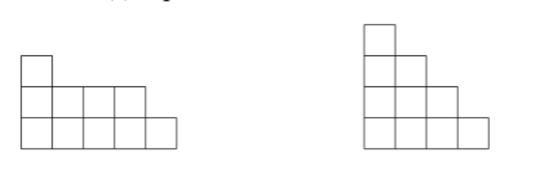
\includegraphics[width=\textwidth]{diag-jung-1}

Очевидно, что множество всех диаграмм Юнга (т.е. «пирамидоподобных» картинок) и неупорядоченных разбиений находятся во взаимно-однозначном соответствии друг с другом.

Биекция часто помогает нам доказывать количества разных вещей в комбинаторике.

\subsubsection{Теорема о количестве неупорядоченных разбиений}
\textbf{Теорема}. Количество неупорядоченных разбиений $n$ на не более, чем $k$ слагаемых равно числу разбиений числа $n+k$ на ровно $k$ слагаемых.

$\\$
\textbf{Доказательство}. Пусть $n=x_1+x_2+\ldots+x_t, t\leqslant k$ --- произвольное разбиение числа $n$ на не более, чем $k$ слагаемых. Ему биективно соответствует некоторая диаграмма Юнга, в которой не более, чем $k$ строчек и ровно $n$ клеток:

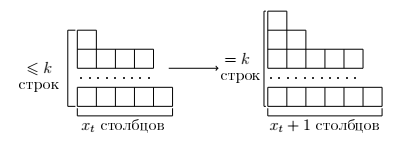
\includegraphics[width=\textwidth]{diag-jung-2}

Приставим к этой диаграмме столбик из $k$ клеточек. Ясно, что это отображение --- также биекция между диаграммами Юнга и при этом, преобразованная диаграмма соответствует некоторому разбиению числа $n+k$ на ровно $k$ слагаемых.

\subsubsection{Двойственная диаграмма Юнга}
Дана диаграмма Юнга некоторого разбиения $n=x_1+x_2+...+x_t,n,x_1,...,x_t \in \mathbb{N}$. Двойственной к ней назовём диаграмму Юнга, в которой число клеток в $i$-й (нумерацию строк и столбцов делаем по убыванию числа клеток) строчке ($1\leqslant i \leqslant x_t$) совпадает с числом клеток в $i$-м столбце первоначальной диаграммы Юнга, а число клеток в $j$-м столбце ($1\leqslant j \leqslant x_t$) двойственной диаграммы Юнга равно числу клеток в $j$-й строчке первоначальной диаграммы Юнга.

Например, следующие две диаграммы двойственны друг другу:

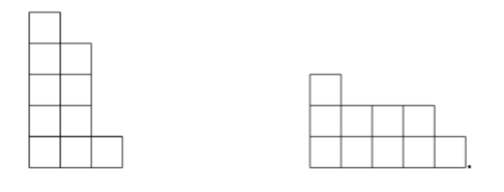
\includegraphics[width=\textwidth]{diag-jung-3}

Легко проверить, что взятие двойственных диаграмм есть биективное отображение множества диаграмм Юнга.

TODO: \textbf{Задача}. Строя двойственные диаграммы Юнга, докажите следующее утверждение: количество неупорядоченных разбиений числа $n$ на слагаемые, каждое из которых не превосходит $k$, равно числу неупорядоченных разбиений числа $n$ на не более, чем $k$ слагаемых.

\subsubsection{Задачи}
\textbf{Задача}. Найдите количество диаграмм Юнга произвольного веса, имеющих не более $p$ строк и не более $q$ столбцов.

$\\$
Представим решетку из $p$ строк и $q$ столбцов. Рассмотрим путь из левого верхнего угла в правый нижний. Возможные пути будут очерчивать возможные варианты диаграмм Юнга. Таким образом, между ними существует биекция (если не учитывать путь по границе, соответствующий пустой диаграмме Юнга).

Изначально может показаться, что количество путей равно $p \times q$, но мы не можем двигаться в любую сторону. Лучше представить это так: всего ходов $p + q$, в какие-то моменты мы поворачиваем вправо. То есть нам нужно выбрать $q$ поворотов вправо из $p + q$ ходов. Тогда итоговое количество будет $C_{p+q}^q$. И так как нужно выкинуть путь по левой и нижней границам (пустая диаграмма Юнга), то итого $C_{p+q}^q - 1$.

$\\$
\textbf{Задача}. Докажите, что количество неупорядоченных разбиений числа $n$ на не более, чем $k$ слагаемых равно количеству неупорядоченных разбиений числа $n+\frac{k(k+1)}{2}$ на $k$ различных слагаемых.

$\\$
Нужно построить биекцию между множествами указанных разбиений, переводя разбиение $(x_1,\ldots,x_l)$, где $x_1 \ge x_2 \ge \ldots \ge x_l$ в разбиение $(x_1+k,\ldots,x_l+(k-l+1),(k-l),\ldots,1)$. Таким образом, вторым разбиением мы всегда доберем ровно до $n+\frac{k(k+1)}{2}$.

$\\$
\textbf{Задача}. Сколькими способами можно разменять купюру в 50 рублей на монеты достоинством 1, 2 и 5 рублей?

$\\$
Распишем по рекурсивной формуле из лекции:
$$\pi(50;1,2,5) =  \pi(45;1,2,5) + \pi(50;1,2) = \pi(40;1,2,5) + \pi(45;1,2) + \pi(50;1,2) = ... $$
$$\pi(50;1,2,5) =\sum\limits_{k=0}^{10} \pi(5k;1,2)$$

Теперь количество слагаемых у нас определяется только единицами и двойками. А если подумать, то только двойками: мы набираем их какое-то количество, а все остальное раскладываем единицами. Теперь разбиваем сумму на числа, кратные $10$ и числа, кратные $5$, но не кратные $10$:
$$\pi(50;1,2,5) =\sum\limits_{l=0}^{5} \pi(10l; 1,2) + \sum\limits_{l=0}^{4}\pi(10l + 5; 1,2) = \sum\limits_{l=0}^{5} (5l+1) + \sum\limits_{l=0}^{4}(5l+3) = 146.$$

$\\$
\textbf{Задача}. Найдите количество упорядоченных разбиений числа 10 на 4 неотрицательных слагаемых. К примеру, есть пять разбиений числа 4 на 2 неотрицательных слагаемых: 4+0, 3+1, 2+2, 1+3, 0+4.

$\\$
Вариант 1. Расставляем перегородки между 10 единичками: 1 + 1 + ... + 1 = 10. Нам нужно расставить 3 перегородки на 11 возможных позиций (+2 из-за того, что мы можем ставить перегородку до первого и после последнего элемента). Кроме того, перегородки могут стоять в одинаковом месте (давая тем самым слагаемое 0). Итого $\overline{C}^{3}_{11}$.

$\\$
Вариант 2. Нам нужно раскидать 10 одинаковых кубиков в 4 разных чашки (соответствующие строкам диаграммы Юнга). Это сочетание с повторением: у нас есть множество из 4 чашек и нам нужно выбрать 10 чашек (с повторением). Получаем $\overline{C}^{10}_{4}$.

$\\$
\textbf{Задача}. Найдите количество всевозможных неупорядоченных разбиений $n=x_1 + \ldots + x_k, 1 \leq n \leq 26, 1 \leq k\leq 7, 1 \leq x_i\leq 4$ (при любых $i$). 

$\\$
сли нарисовать диаграмму Юнга, соответствующую данному разбиению, то это почти все диаграммы, содержащие не более 7 строк и не более 4 столбцов. ``Почти'', потому что надо выбросить пустую диаграмму и ещё две, дающие в сумме 27 и 28. Итого $C_{11}^4 - 3= 327$.

$\\$
\textbf{Задача}. Сколькими способами можно оплатить посылку за 19 копеек марками достоинством 1,4,6 или 10 копеек? (Порядок марок не важен).

$\\$
Считаем руками (при этом помним, что удобно дойти до $\pi(n;1,4) = \left[\frac{n}{4}\right]+1$: 4 может попасться от 0 до $\left[\frac{n}{4}\right]$ раз, остальное забиваем единицами). Также удобно строить дерево ветвлений рекурсии, помечая ребра количеством вариантов и добираясь от листьев до корня. В итоге получится 16.

$\\$
\textbf{Задача}. Найдите количество упорядоченных разбиений числа 19 на ровно пять слагаемых, которые равны 1,4,6,10.

$\\$
Считаем руками. На удивление выходит только 2 разбиения: 10 + 6 + 1 + 1 + 1 и 6 + 4 + 4 + 4 + 1. Каждый из вариантов разветвляется из-за упорядоченности на $P(3,1,1) = 20$. В итоге 40. 

\section{Линейные рекуррентные соотношения. Формальные степенные ряды}
\subsection{Линейные рекуррентные соотношения с постоянными коэффициентами}
\subsubsection{Общее определение}
Возьмем числа $a_0, a_1,...a_k  \in  \mathbb{C};, a_k\ne 0, a_0 \ne 0$.

Последовательность чисел $y_0,y_1,...,y_n ...$ удовлетворяет линейному рекуррентному соотношению $k$-ого порядка с коэффициентами $a_0, a_1...,a_k$, если для любого $n$ выполняется равенство:
$$a_k y_{n+k}=a_{k-1}y_{n+k-1}+...+a_1y_{n+1}+a_0 y_n$$

Выражение является линейным. Как видно, $a_k$ в данном выражении не играет роли, поэтому на него можно сократить.

\subsubsection{Числа Фибоначчи}

Числа Фибоначчи --- это типичное линейное рекуррентное соотношение: $F_n=F_{n-1}+F_{n-2}, k=2$. Начальные условия: $F_0 = 0, F_1 = 1$.

\subsubsection{Линейные рекуррентные соотношения второго порядка. Характеристическое уравнение}

Линейные рекуррентные соотношения второго порядка выражаются общей формулой: 
$$y_{n+2}=a_1 y_{n+1}+a_0y_n, a_0 \ne 0. ~~~~~(*)$$

Можно записать для него так называемое характеристическое уравнение:
$$\lambda ^2=a_1\lambda+a_0.$$
Пусть $\lambda_1, \lambda_2$ --- корни этого характеристического уравнения (у любого квадратного уравнения есть два корня, просто они могут быть комплексными или совпадать).

\subsubsection{Теоремы}
\textbf{Теорема 1}. Пусть $\lambda_1\ne \lambda_2$. Тогда:

1. Для любых чисел $C_1,C_2 \in \mathbb{C}$ последовательность $y_n = C_1 \lambda_1^n+C_2\lambda_2^n$ удовлетворяет рекуррентному соотношению $(*)$.

2. Пусть $y_n$ --- последовательность чисел, удовлетворяющих $(*)$. Тогда существуют такие числа $C_1,C_2 \in \mathbb{C}$, что $y_n = C_1 \lambda_1^n+C_2\lambda_2^n$.

$\\$
\textbf{Доказательство 1 пункта}.

Возьмём произвольные $C_1, C_2$ и рассмотрим $y_n = C_1 \lambda_1^n+C_2\lambda_2^n$.

Мы знаем, что $y_{n+2}=C_1\lambda_1^{n+2}+C_2\lambda_2^{n+2}$ и $y_{n+1}=C_1\lambda_1^{n+1}+C_2\lambda_2^{n+1}$. Подставим их $(*)$:
$$C_1\lambda_1^{n+2}+C_2\lambda_2^{n+2}-a_1(C_1\lambda_1^{n+1}+C_2\lambda_2^{n+1})-a_0(C_1\lambda_1^{n}+C_2\lambda_2^{n})=$$
$$= C_1\lambda_1^n(\lambda_1^2-a_1\lambda_1-a_0)+C_2\lambda_2^n(\lambda_2^2-a_1\lambda_2-a_0)=0.$$
Поскольку $\lambda_1, \lambda_2$ --- корни характеристического уравнения, то выражения в скобках равны нулю.

$\\$
\textbf{Доказательство 2 пункта}.

Пусть $y_0, y_1,...,y_n,...$ удовлетворяет пункту $(*)$. Составим систему уравнений:
$$\begin{cases} C_1+C_2=y_0\\ C_1\lambda_1+C_2\lambda_2=y_1  \end{cases}$$
Эта система относительно $C_1$ и $C_2$, поскольку $y_0, y_1, \lambda_1, \lambda_2$ известны. Эта система разрешима, так как определитель равен $\lambda_2 - \lambda_1 \ne 0$. Следовательно, $C_1$ и $C_2$ --- решение системы.

Рассмотрим последовательность $y_n^*=C_1\lambda_1^n+C_2\lambda_2^n$ (которая также удовлетворяет $(*)$). Заметим, что:
$y_0^*=C_1+C_2=y_0$

$y_1^*=C_1\lambda_1+C_2\lambda_2=y_1$

И так как $y_n$ и $y_n^*$ связаны одинаковым рекуррентными соотношением и у них одинаковые начальные члены, то для любого $n$ выполняется $y_n = y_n^*$.

$\\$
\textbf{Теорема 2}.  Пусть $\lambda_1= \lambda_2 = \lambda$. Тогда:

1. Для любых чисел $C_1,C_2 \in \mathbb{C}$ последовательность $y_n=(C_1n+C_2) \lambda^n$ удовлетворяет рекуррентному соотношению $(*)$.

2. Пусть $y_n$ --- последовательность чисел, удовлетворяющих $(*)$. Тогда существуют такие числа $C_1, C_2$, что $y_n=(C_1n+C_2) \lambda^n$.

TODO: доказать (доказывается аналогично, а брать прежнюю комбинацию мы не могли потому, что у нас система получится неразрешимой).

\subsubsection{Линейные рекуррентные соотношения $k$-ого порядка}
Общая формула:
$$y_{n+k}=a_{k-1}y_{n+k-1}+...+a_1y_{n+1}+a_0y_n, a_0 \ne 0.~~~(**)$$
Характеристическое уравнение:
$$\lambda^k = a_{k-1}\lambda^{k-1}+...+a_1\lambda+a_0.$$

$\\$
\textbf{Основная теорема алгебры (б/д)}. Любой многочлен с коэффициентами из $\mathbb{C}$ имеет хотя бы один корень в $\mathbb{C}$.

\textbf{Следствие}. Многочлен $k$-ой степени имеет ровно $k$ корней (с учетом кратности).

Введем $\lambda_1, \lambda_2,...,\lambda_k \in \mathbb{C}$ --- корни характеристического уравнения.

Введем $\mu_1,...,\mu_r$ --- различные числа в множестве $\{\lambda_1, \lambda_2,...,\lambda_k\}$.

Введем $k_1,...,k_r$, где $k_i$ --- количество $\lambda_i$, равных $\mu_i$. Тогда $k_1+...+k_r=k$.

$\\$
\textbf{Теорема}. 
1. Пусть:

- $P_1(n)$ --- произвольный многочлен степени, меньшей или равной $k_1 - 1$;

- $P_2(n)$ --- произвольный многочлен степени, меньшей или равной $k_2 - 1$;

- $P_r(n)$ --- произвольный многочлен степени, меньшей или равной $k_r - 1$;

Тогда последовательность $y_n=P_1(n)\mu_1^n+P_2(n)\mu_2^n+\ldots+P_r(n)\mu_r^n$ удовлетворяет соотношению $(**)$.

2. Пусть $y_n$ удовлетворяет $(**)$. Тогда существует $P_1(n),...,P_r(n) : \forall i ~ degP_i(n)\le k_i-1$ и $y_n =P_1(n)\mu_1^n+...+P_r(n)\mu_r^n$.

TODO: доказать (доказывается так же, только нужно возиться с определителями).

TODO: все равно это все какой-то магией для меня выглядит.
$\\$
Из этой теоремы можно получить теорему для рекуррентных соотношений второго порядка, если просто аккуратно все подставить.

\subsubsection{Задачи}
\textbf{Задача}. Найдите формулу $n$-ого числа для последовательности $y_n$, заданной соотношениями $y_0=0,y_1=1, y_{n+2}=y_{n+1}+y_n$ ( числа Фибоначчи ).

$\\$
Тупо подставляем и считаем все по формулам. Например, для чисел Фибоначчи.

Характеристическое уравнение: $\lambda^2- \lambda - 1 =0$. Корни $\lambda_{1},\lambda_2 = \frac{1\pm \sqrt{5}}{2}$.

Следовательно, $y_n = C_1 \left(\frac{1+ \sqrt{5}}{2}\right)^n + C_2\left( \frac{1- \sqrt{5}}{2}\right)^n$. Находим $C_0$ и $C_1$ с помощью начальных условий:
$$\begin{cases} C_1 + C_2 = 0, \\ C_1 \frac{1 + \sqrt{5}}{2} + C_2 \frac{1 - \sqrt{5}}{2} = 1.\end{cases} \Leftrightarrow \begin{cases} C_1 = -C_2, \\ 1=C_1(\frac{1 + \sqrt{5}}{2}-\frac{1 - \sqrt{5}}{2})=C_1(2\frac{\sqrt{5}}{2}) =\sqrt{5}C_1.\end{cases} \Leftrightarrow \begin{cases} C_1 = -C_2, \\ C_1 = \frac{1}{\sqrt{5}}.\end{cases}$$

В итоге получаем:
$$y_n = \frac{1}{\sqrt{5}} \left(\frac{1+ \sqrt{5}}{2}\right)^n -\frac{1}{\sqrt{5}} \left( \frac{1- \sqrt{5}}{2}\right)^n$$.

Нужно просто все аккуратно подставлять и считать.


$\\$
\textbf{Задача}.Какому рекуррентному соотношению 2-ого порядка удовлетворяет последовательность

а) $y_n=n$;

б) $y_n=2^n+2$?

$\\$
Нужно просто решить все в обратном порядке. Например, для а) мы видим, что $\lambda_1 = \lambda_2 = 1$, $C_1 = 1, C_2 = 0$.

$\\$
\textbf{Задача}. Пусть $s_n$ --- количество таких подмножеств $A$ множества $\{1,2,...,n\}$, что для любых двух различных элементов $a,b \in A$ выполнено неравенство $|a-b| \geq 2$. Найдите $s_15$.

$\\$
Мы хотим найти рекуррентное соотношение на $s_n$. Рассмотрим два случая.

1. Пусть $n \not \in A$. Тогда $A$ является подмножеством множества $\{1,2,...,n-1\}$, удовлетворяющим данному условию. Количество таких подмножеств равно $s_{n-1}$.

2. Предположим теперь, что $n \in A$. Тогда по нашему условию $n-1 \not \in A$, а оставшееся множество $A \setminus \{n\}$ является подмножеством множества $\{1,2,...,n-2\}$, удовлетворяющим нашему условию. Значит, всего таких множеств $s_{n-2}$.

Таким образом, мы получаем рекуррентное соотношение $s_n=s_{n-1}+s_{n-2}$. Это в точности рекуррентное соотношение для чисел Фибоначчи. Найдём начальные члены нашей последовательности. $s_0=1$ (пустое подмножество), $s_1=2$ (подмножества $\emptyset$, $\{1\}$). Так как $s_0=F_2, s_1=F_3$ и рекуррентные соотношения у последовательностей $s_n$ и $F_n$ совпадают, мы получаем равенство $s_n=F_{n+2}$. Следовательно, $s_{15}=F_{17}=1597$.

$\\$
\textbf{Задача}. Лягушка прыгает по вершинам шестиугольника $ABCDEF$, перемещаясь каждый раз в одну из соседних вершин. Обозначим через $A_n$ количество способов, которыми Лягушка может попасть из $A$ в $A$ за $n$ прыжков.

а) Найдите рекуррентное соотношение для последовательности $A_n$.

б) Найдите значение $A_n$.

$\\$
Очевидно, что за нёчетное количество шагов из $A$ можно попасть только в $B$, $D$ и $F$. Поэтому, $A_{2n+1}=0$. Пусть теперь $n$ --- чётное число. Введём дополнительные последовательности $C_n$ и $E_n$ для количества способов попасть из $A$ в $C$ и $E$ соответственно. Заметим, что из симметрии задачи следует, что $C_n=E_n$. Тогда:

$A_n = 2A_{n-2} + C_{n-2}+E_{n-2} = 2A_{n-2} + 2C_{n-2}$

$C_n = A_{n-2} + 2C_{n-2} + E_{n-2} = A_{n-2}+3C_{n-2}$

Найдём отсюда рекуррентное соотношение для $A_n$: 
$$\begin{cases} A_n = 2A_{n-2} + 2C_{n-2}, \\ C_n = A_{n-2}+3C_{n-2} \end{cases} \Leftrightarrow \begin{cases} 2C_{n-2} = A_n -2A_{n-2} , \\ A_{n+2} - 2A_{n} = 2A_{n-2}+3(A_n - 2A_{n-2}) \end{cases} \Rightarrow A_{n+2} - 5A_{n} + 4A_{n-2}=0.$$

Обозначим $A’_n = A_{2n}$, для которой мы имеем рекуррентное соотношение: $A’_{n+1} = 5A’_{n} - 4A’_{n-1}$.

Найдем для него характеристическое уравнение: $\lambda^2 - 5\lambda + 4 = 0$, корни равны 1 и 4.

Следовательно, $A’_n = C_1\cdot 1^n + C_2 \cdot 4^n$. Подставим значения $A’_1=A_2=2, A’_2=A_4=6$ и найдем $C_1 = \frac{2}{3}, C_2 = \frac{1}{3}$. В итоге имеем $A_{2n} = \frac{2+4^n}{3}$.

$\\$
То есть, рекуррентное соотношение нам позволяет вообще не думать о переборе вариантов, мы просто устанавливаем зависимость между последними двумя членами (для порядка 2). При этом стоит понимать, что действительно нам достаточно только последних двух.

\subsection{Формальные степенные ряды}
\subsubsection{Общее определение}
Пусть даны числа $a_0, a_1, a_2,...,a_n,... \in \mathbb{R}$ (хотя комплексные тоже могут быть).

Назовём формальным степенным рядом с коэффициентами $a_0,a_1,...$ следующую "картинку":
$$a_0+a_1x+a_2x^2+...+a_nx^n+...$$
Здесь мы не придаем значения тому, что может быть $x$-ом, мы даже не считаем это функцией аргумента, для нас это просто крестик.

$\\$
\textbf{Сумма формальных степенных рядов}.

Пусть $A$ и $B$ --- формальные степенные ряды. Тогда их суммой называется формальный степенной ряд $C=C_0+C_1x+...+C_nx_n+...$, у которого $\forall i c_i=a_i+b_i$.

TODO: откуда такая формула?!

ANSWER: такая вот формула для произведения многочленов например --- можно взять листочек и ручку и попробовать перемножить $(a_0 + a_1x + a_2x^2)(b_0 + b_1x + b_2x^2)$. В итоге получится, что коэффициент при $x^0$ --- это $a_0b_0$, при $x^1$ --- $(a_0b_1 + a_1b_0)$, при $x^2$ --- $(a_0b_2 + a_1b_1 + a_2b_0)$ и так далее прямо по этой формуле.

TODO: доказательство формулы?

$\\$
\textbf{Умножение формальных степенных рядов}.

Пусть $A$ и $B$ --- формальные степенные ряды. Тогда их произведением называется формальный степенной ряд $C=C_0+C_1x+...+C_nx_n+...$, у которого $\forall i$:
$$C_i=\sum\limits_{j=0}^i a_jb_{i-j}$$

\textbf{Деление формальных степенных рядов}.

Пусть $A$ и $B$ --- формальные степенные ряды. $C=A/B \Leftrightarrow ~A=BC$:
$$\begin{cases} a_0=b_0c_0\\ a_1=b_1c_0+b_0c_1 \\a_2=b_2c_0+b_1c_1+b_0c_2 \\ ...\end{cases}$$

Достаточным условием для делимости является $b_0 \ne 0$: тогда система будет иметь решение.

$\\$
Например, для рядов $A=1,B=1-x$ имеем (с помощью деления в столбик):

$$\frac{1}{1-x}=1+x+x^2+x^3+...+x^n+...$$

То есть, деля в столбик мы фактически решаем вышеприведенную систему уравнений (TODO: wow).

\subsubsection{Вывод комбинаторного тождества при помощи формальных степенных рядов}

$\frac{1}{(1-x^2)^2}=\left( \frac{1}{1-x} \right)^2 \cdot \left( \frac{1}{1+x} \right)^2$ --- формальный степенной ряд.

Можно получить ряд с помощью такого преобразования:
$$\left( \frac{1}{1-x^2} \right)^2= \left( 1+x^2+x^4+...+x^{2n}+...\right)^2=1+2x^2+3x^4+...+(n+1)x^{2n}+...$$

Теперь попробуем поделить изначальное выражение:
$$\left( 1+x+x^2+...+x^{n}\right)^2 \left( 1-x+x^2-...+(-1)^nx^{n}+\right)^2=$$
$$=\left(1+2x+3x^2+...+(n+1)x^{n}+...\right) \left(1-2x+3x^2-...+(-1)^n(n+1)x^{n}+...\right)=$$
$$=...+x^n\left(1\cdot(-1)^n(n+1)+2\cdot(-1)^{n-1}n+...+(n+1)\cdot(-1)^0\cdot1\right)+...~,$$
И получается, что этот монструозный коэффициент в скобках равен тому, что мы уже нашли:
$$\begin{cases} k+1 , n=2k\\ 0,n=2k+1\end{cases}.$$
Таким образом, мы вывели комбинаторное тождество (так как не предъявляли никаких требований к $x$). TODO: не очень я это понял.

\subsubsection{Задачи}
\textbf{Задача}. Пусть $F=1+x+x^2+\ldots$, $G=1-x+x^2-x^3+\ldots$. Найти $F + G, F \cdot G$.

$\\$
По определению умножения получаем:

$F+G = 2+ 2x^2 + 2x^4 + \ldots$

$F \cdot G = 1 + x^2 + x^4 + \ldots$

$\\$
\textbf{Задача}. Пусть $F = \sum_{k=0}^{\infty} \frac{1}{k!}x^k$, $G = \sum_{k=0}^{\infty} \frac{(-1)^k}{k!}x^k$, найти $F \cdot G$, $F^2$.

$\\$
Пусть $F \cdot G = \sum_{k=0}^{\infty} a_k x^k$. Тогда по определению умножения:
$$a_k = \sum_{i=0}^k \frac{1}{i!} \cdot \frac{(-1)^{k-i}}{(k-i)!} =\frac{1}{k!} \sum_{i=0}^k \frac{k!(-1)^{k-i}}{i!(k-i)!} = \frac{1}{k!} \sum_{i=0}^k  C_k^i (-1)^{k-i} = \begin{cases} \frac{1}{k!}, k=0 \\ 0, k \neq 0. \end{cases}  =  \begin{cases}1, k=0 \\ 0, k \neq 0 \end{cases}$$
Вот таким вот трюком мы превратили это в бином Ньютона.

$\\$
Теперь найдем $F^2 = \sum_{k=0}^{\infty} b_k x^k$:
$$b_k = \sum_{i=0}^k \frac{1}{i!} \cdot \frac{1}{(k-i)!} =\frac{1}{k!} \sum_{i=0}^k \frac{k!}{i!(k-i)!} = \frac{1}{k!} \sum_{i=0}^k  C_k^i = \frac{2^k}{k!},$$
И снова тот же трюк и бином Ньютона.

$\\$
\textbf{Задача}. Найдите коэффициенты $\frac{1}{(1-x)}$.

$\\$
Это можно решить с помощью деления в столбик или системы уравнений. Рассмотрим решение с помощью системы линейных уравнений.

Пусть $\frac{1}{(1-x)} = \sum_{k=0}^{\infty} c_k x^k$. Переделаем выражение:

$$1 = (1-x) \cdot \sum_{k=0}^{\infty} c_k x^k = (1 -x)(c_0 + c_1x + c_2x^2 +...)$$.

Не забываем, что это произведение двух формальных степенных рядов.
$$\begin{cases} 1 = c_0;\\ 0 =c_1-c_0; \\ 0 = c_2-c_1; \\ \ldots  \end{cases}.$$
Решая ее, получаем $1=a_0=a_1=a_2=\ldots$, следовательно $\frac{1}{1 -x} = 1 + x + x^2 + x^3 +...$

$\\$
\textbf{Задача}. Найдите коэффициенты $\frac{1}{(2-x)}$.

$\\$
Алгоритм деления в столбик (уголком) очень простой: нам нужно каждый раз вычитать из того, что у нас на данный момент имеется или остается некоторое произведение. Произведение состоит из делителя и выражения, которое подобрано таким образом, чтобы погасить самую большую часть нашего делимого. Именно это выражение мы и добавляем в ответ.

$\\$
Разделим $\frac{1}{2-x}$. На какое выражение мы должны домножить $2 - x$, чтобы погасить единицу? На $\frac{1}{2}$. Вычитаем $\frac{1}{2}(2 -x) = 1 - \frac{x}{2}$. Остается $\frac{x}{2}$. Нужно погасить $\frac{x}{2}$. Вычитаем $\frac{x}{4}(2-x)$. Остается $\frac{x}{4}$. И так далее. В итоге получается $\frac{1}{2} + \frac{x}{4} + \frac{x^2}{8} + ...$

$\\$
\textbf{Задача}. Найдите коэффициенты $\frac{1}{(1-x)^m}$.

$\\$
Нам нужно найти коэффициенты ряда $(1 + x + x^2 + x^3 + ...)^m$. Как мы можем получить степени $x^k$? На помощь приходят шарики и перегородки! Шарики --- это порядок $k$, который нам нужно шабрать, перегородки --- степень, которая берется из каждой "скобки": $x^0, x^1, x^2,...$. Таким образом, у нас есть $m$ скобок, что дает в распоряжении $m-1$ перегородок. Мы можем поставить их на $k+1$ место. Таким образом, нам $m-1$ раз нужно вытащить "место" из $k+1$ возможных, что дает $a_k = \overline{C}_{k+1}^{m-1} = C_{m+k-1}^{m-1}$.

$\\$
\textbf{Задача}. Найдите коэффициенты $\frac{1}{(1-x)(2-x)}$.

$\\$
Можно перемножить предыдущие дроби, а можно решить иначе. Сведём одну дробь со сложным знаменателем к двум простым дробям: запишем формальное равенство $\frac{1}{(1-x)(2-x)} = \frac{A}{1-x} + \frac{B}{2-x}$ и попробуем подобрать $A$ и $B$.

$$\frac{A}{1-x} + \frac{B}{2-x} = \frac{A(2-x) + B(1-x)}{(1-x)(2-x)} = \frac{ x (-A-B)+ (2A+B)}{(1-x)(2-x)} = \frac{1}{(1-x)(2-x)} \Rightarrow x (-A-B)+ (2A+B) = 1 \Leftrightarrow$$

$$\Leftrightarrow \begin{cases} -A-B =0 ,\\ 2A+B=1 \end{cases} \Leftrightarrow \begin{cases} A =1 ,\\ B=-1 \end{cases},$$
Отсюда:
$$\frac{1}{(1-x)(2-x)} = \frac{1}{1-x} - \frac{1}{2-x} = (1+x+x^2+x^3+ \ldots) - (\frac{1}{2} + \frac{1}{4} x + \frac{1}{8}x^2 + \ldots) = \sum_{k=0}^{\infty}(1- \frac{1}{2^{k+1}})\cdot x^k.$$ 

$\\$
\textbf{Задача}. Даны ряды:
$$S(x) = \sum\limits_{n=0}^{\infty} \frac{(-1)^n}{(2n+1)!} x^{2n+1}, C(x) = \sum\limits_{n=0}^{\infty} \frac{(-1)^n}{(2n)!} x^{2n}.$$
Найти коэффициент при $x^{2014}$ ряда $S^2(x)+C^2(x)$.

$\\$
Коэффициент при $x^{2014}$ у ряда $S^2(x)$ равен:
$$\sum_{n=0}^{1006} \frac{(-1)^n}{(2n+1)!} \frac{(-1)^{1006-n}}{(2014-(2n+1))!}= \frac{1}{2014!}\sum_{n=0}^{1006} \frac{2014!}{(2n+1)!(2014-(2n+1))!} = \frac{1}{2014!}\sum_{n=0}^{1006} C_{2014}^{2n+1}$$

Аналогично, коэффициент при $x^{2014}$ у ряда $C^2(x)$ равен:
$$\sum_{n=0}^{1007} \frac{(-1)^n}{(2n)!} \frac{(-1)^{1007-n}}{(2014-2n)!} =\frac{-1}{2014!} \sum_{n=0}^{1007} \frac{2014!}{(2n)!(2014-2n)!}= \frac{-1}{2014!}\sum_{n=0}^{1007} C_{2014}^{2n}$$

Итого, сумма коэффициентов равна:
$$\frac{-1}{2014!}\sum_{n=0}^{1007} C_{2014}^{2n} + \frac{1}{2014!}\sum_{n=0}^{1006} C_{2014}^{2n+1} = \frac{-1}{2014!}\sum_{n=0}^{2014} C_{2014}^n (-1)^{n} =0$$

$\\$
\textbf{Задача}. Сколько существует строк из 12 нулей и единиц, в каждой из которых никакие два нуля не стоят рядом?

$\\$
Обозначим через $a_n$ количество строк из $n$ нулей и единиц, в каждой из которых никакие два нуля не стоят рядом.

Рассмотрим последнее число в строке. Если оно равно $1$, то на первых $n-1$ местах может стоять любая строка, удовлетворяющая нашему условию. Следовательно, их количество равно $a_{n-1}$. Если на последнем месте стоит $0$, значит, на $n-1$ месте стоит $1$, а на первых $n-2$ местах стоит любая строка, удовлетворяющая нашему условию. Поэтому количество таких строк равно $a{n-2}$.

Мы получили рекуррентное соотношение на $a_n: a_n=a_{n-1}+a{n-2}$. Начальные члены этой последовательности равны $a_1=2, a_2=3$. Следовательно, последовательность $a_n=F_n+2$, где $F_n$ --- последовательность чисел Фибоначчи. Поэтому $a_{12}=F_{14}=377$.

$\\$
\textbf{Задача}. Лягушка прыгает по вершинам пятиугольника $ABCDE$, перемещаясь каждый раз в одну из соседних вершин. Обозначим через $K_n$ количество способов, которыми лягушка может попасть из $A$ в $B$ за $n$ прыжков. Найдите характеристический многочлен рекуррентного соотношения для последовательности $K_n$.

$\\$
Обозначим через $X_n$ количество способов попасть из вершины $A$ в вершину $X$ за $n$ прыжков соответственно. Исходя из симметрии, получаем, что $B_n=E_n, C_n=D_n$. Нам необходимо найти $B_n$. Имеем следующие соотношения:
$$\begin{cases} A_n = 2B_{n-1}, \\ B_n = A_{n-1} + C_{n-1}; \\ C_n = B_{n-1} + C_{n-1}. \end{cases} \Leftrightarrow \begin{cases} A_n = 2B_{n-1}, \\ B_n = 2B_{n-2} + C_{n-1}; \\ C_n = B_{n-1} + C_{n-1}. \end{cases} \Rightarrow$$
$$\begin{cases} C_{n} = B_{n+1}- 2B_{n-1}; \\ C_n = B_{n-1} + C_{n-1}. \end{cases} \Rightarrow B_{n+1}- 2B_{n-1} = B_{n-1} + (B_{n}- 2B_{n-2}).\Leftrightarrow$$
$$\Leftrightarrow B_{n+1}- B_n - 3B_{n-1} + 2B_{n-2} = 0.$$

$\\$
\textbf{Задача}. Найдите коэффициент при $x^5$ у степенного ряда $(1-2x+4x^2-8x^3+\ldots+(-2)^k x^k+\ldots)^{10}$.

$\\$
Данный ряд получается подстановкой степенного ряда $-2x$ в $(1+x+x^2+x^3+\ldots)$.

А мы знаем, что $(1+x+x^2+x^3+\ldots)^{10} = \sum\limits_{n=0}^{\infty} C_{10+n-1}^{n}x^n$. Следовательно:

$$(1-2x+4x^2-8x^3+\ldots)^{10} = \sum\limits_{n=0}^{\infty} C_{10+n-1}^{n}(-2x)^n.$$ TODO: не понял этого.

Таким образом, коэффициент при $x^5$ равен $C_{14}^5\cdot (-2)^5 = 2002 \cdot(-32)=-64064$.

Таким образом, на ряды очень удобно смотреть через призму разложения на множители.

$\\$
\textbf{Задача}. Найдите коэффициент при $x^{10}$ степенного ряда $\frac{x}{(1-2x)(1-3x)}$

$\\$
Разбиваем на слагаемые с коэффициентами в числителе, решаем систему уравнений, подставляем, получаем сумму двух дробей, представляем их в виде суммы двух рядов, считаем сумму, получаем ответ 58025. Все стандартно.

\section{Производящие функции}
\subsection{Производящие функции}
\subsubsection{Общее определение}
Производящей функцией последовательности чисел $a_0,a_1,...,a_n,...$ ($\in \mathbb{C}$) называется формальный степенной ряд, коэффициенты которого образуют заданную последовательность чисел:
$$f(x)=\sum\limits_{k=0}^\infty a_k x^k$$

Его частичными суммами называются конечные ряды:
$$S_n(x)=\sum\limits_{k=0}^n a_k x^k$$

Функция $f(x)$ определена в точке $x$, если существует $\lim_{n \to \infty}S_n(x)$. Значение этого предела по определению есть значение ряда в точке $x$.

\subsubsection{Теорема о сходимости рядов}
\textbf{Теорема о сходимости рядов}.

Пусть $\rho =\frac{1}{\overline{\lim}_{n \to \infty} \sqrt[n]{|a_n|}}$ (``$\overline{\lim}_{n \to \infty}$'' --- это верхний предел, супремум).

Тогда функция $f(x)=\sum\limits_{k=0}^\infty a_k x^k$ определена в каждой точке $x~:~|x| < \rho$, где $\rho$ --- радиус сходимости ряда. $\rho$ называется радиусом, потому что если рассматривать $x$ на комплексной плоскости, то там конечно круг. А если на вещественной прямой --- то да, понятие радиуса избыточно, потому что мы просто не вылезаем за пределы интервала.

TODO: доказательство теоремы.

$\\$
\textbf{Пример 1}. Пусть $a_n = $. Тогда $f(x)=\sum\limits_{n=0}^\infty x^n$. Действительно, в этом ряду коэффициенты при всех степенях $x$ равны $1$, а значит, $\rho=1$. По теореме ряд определён при $|x|<\rho$; следовательно, ряд сходится при $|x|<1$.

$\\$
\textbf{Пример 2}. Пусть теперь $f(x) = \begin{cases} 2^n,~n~-~\text{четное};\\ 3^n,~n~-~\text{нечетное}. \end{cases}$. Здесь есть две подпоследовательности: $2^nx^n$ и $3^nx^n$. Имеем $\sqrt[n]{|2^n|}=2, \sqrt[n]{|3^n|}=3.$. Очевидно, верхним пределом будет $3$, значит, ряд сходится при $|x| < \frac{1}{3}$.

\subsubsection{Сходимость на границе круга}
Посмотрим на ряд $\sum\limits_{n=1}^\infty \frac{x^n}{n},~\rho =\frac{1}{\overline{\lim}_{n \to \infty} \sqrt[n]{|\frac{1}{n}|}}=1$. При $x=1$ ряд расходится, а при $x=-1$ --- сходится (по признаку Лейбница).

$\\$
С рядом $\sum\limits_{n=1}^\infty \frac{x^n}{n^2}$. Для него основа $\rho = 1$. Однако ряд сходится при обоих значениях $x = \pm 1$. При этом $\sum\limits_{n=1}^\infty \frac{1}{n^2}=\frac{\pi^2}{6}.$

\subsubsection{Задачи}
\textbf{Задача}. Вычислить сумму $\sum\limits_{k=0}^n C^k_n\cdot k^2 \left(\frac{2}{3}\right)^k.$

$\\$
Рассмотрим функцию $f(x)=\sum\limits_{k=0}^n C^k_n\cdot x^k ~$ --- производящую функцию последовательности $C_n^0,C_n^1,...,C_n^n.$ Для нее мы знаем сумму: $f(x)=\sum\limits_{k=0}^n C^k_n\cdot x^k =(1+x)^n$ (бином Ньютона).

Тогда имеем:

$$f'(x)=\sum\limits_{k=1}^n kC^k_n\cdot x^{k-1},$$

$$xf'(x)=\sum\limits_{k=1}^n kC^k_n\cdot x^k,$$

$$\left( x f'(x)\right)'=\sum\limits_{k=1}^n k^2 C^k_n\cdot x^{k-1},$$

$$x\left( x f'(x)\right)' |_{x=\frac{2}{3}} = \sum\limits_{k=0}^n C^k_n\cdot k^2 \left(\frac{2}{3}\right)^k.$$

В итоге имеем:
$$x\left( x f'(x)\right)'=\left( n(1+x)^{n-1}x\right)'\cdot x.$$

$\\$
\textbf{Задача}. Чему равен $\overline{\lim}_{n\to \infty} \sqrt[n]{|a_n|}$, где $a_n = n^2$.

$\\$
Докажем, что для всех достаточно больших n выполнено неравенство $\sqrt[n]{n^2}<1+x$, где $x > 0$ --- произвольное число. Имеем:
$$\sqrt[n]{n^2} < 1+x \Leftrightarrow n^2 < (1+x)^n \Leftrightarrow n^2 < 1+C_n^1 x + C_n^2 x^2 +\ldots + C_n^n x^n$$
Ослабим неравенство:
$$n^2 < C_n^3 x^3 = \frac{n(n-1)(n-2)}{6}x^3 \Leftrightarrow n < \frac{1}{6}(n-1)(n-2) x^3 \Leftrightarrow \frac{n}{n-1} < \frac{1}{6} (n-2)x^3.$$

Если взять $n > \frac{12}{x^3}+2$, то $(n-2) > \frac{12}{x^3} \Leftrightarrow \frac{1}{6}(n-2)x^3 > 2 > \frac{n}{n-1} \Rightarrow \sqrt[n]{n^2} < 1+x$.

Следовательно, для любого $x > 0$ выполняется $\sqrt[n]{n^2} < 1+x$ при всех достаточно больших $n$.

Также очевидно, $\sqrt[n]{n^2} \geqslant 1$ при всех $n$. Таким образом, $\lim_{n \to \infty} a_n =1$. TODO: а не $\lim_{n\to \infty} \sqrt[n]{|a_n|}$?

TODO: Кажется, было проще просто посчитать предел $n^{\frac{2}{n}}$.

$\\$
\textbf{Задача}. Чему равен $\overline{\lim}_{n\to \infty} \sqrt[n]{|a_n|}$, где $a_n = \lambda_1^n + \lambda_2^n$.

$\\$
Пусть $|\lambda_1| \le |\lambda_2|$.

Если $\lambda_1=\lambda_2=0$, то $a_n = 0$ и верхний предел также равен $0$.

Если $\lambda_2 \ne 0$. Докажем, что для любого положительного $x$ при всех достаточно больших $n$ выполнено неравенство:
$$\frac{ \sqrt[n]{|\lambda_1^n + \lambda_2^n|}}{|\lambda_2|} < 1+x$$

Мы знаем, что:
$$\frac{ \sqrt[n]{|\lambda_1^n + \lambda_2^n|}}{|\lambda_2|} \leqslant \sqrt[n]{\frac{|\lambda_1|^n}{|\lambda_2|^n} + 1}.$$

Введем обозначение $y = \frac{|\lambda_1|}{|\lambda_2|}$. Получаем:
$$\sqrt[n]{y^n+1} < 1+x \Leftrightarrow y^n+1 < (1+x)^n = 1+C_n^1 x + \ldots + C_n^n x^n \Leftarrow y^n < nx .$$

Значит, для любого натурального $n$, большего, чем $\frac{x}{y}$, выполнены неравенства:
$$\frac{ \sqrt[n]{|\lambda_1^n + \lambda_2^n|}}{|\lambda_2|} \leqslant \sqrt[n]{y^n+1} < \sqrt[n]{y+1} <\sqrt[n]{nx+1} < \sqrt[n]{(1+x)^n} = 1+x.$$
С другой стороны,
$$\frac{ \sqrt[n]{|\lambda_1^n + \lambda_2^n|}}{|\lambda_2|} \geqslant \frac{ \sqrt[n]{|\lambda_2|^n - |\lambda_1|^n|}}{|\lambda_2|} = \sqrt[n]{1 -y^n} \ge 1-y^n.$$
При этом,
$1-y^n \ge 1-x \Leftrightarrow y^n \le x \Leftrightarrow \left(\frac{1}{y}\right)^n > \frac{1}{x}$

Из решения предыдущей задачи следует, что $a^n > n^2$, $a > 1$.

Значит, $\left(\frac{1}{y}\right)^n > n^2 > \frac{1}{x}$.

Значит, для любого $x>0$ найдётся $n$ такое, что
$$\frac{ \sqrt[n]{|\lambda_1^n + \lambda_2^n|}}{|\lambda_2|} \ge 1-y^n \geqslant 1-x$$
Следовательно, $\lim_{n\to \infty} \frac{ \sqrt[n]{|\lambda_1^n + \lambda_2^n|}}{|\lambda_2|} = 1$, откуда $\lim_{n\to \infty} \sqrt[n]{|\lambda_1^n + \lambda_2^n|}= |\lambda_2|$.

TODO: ничего не понял.

$\\$
\textbf{Задача}. Как выглядит производящая функция для числа способов набрать n рублей монетами достоинством 1, 2 и 5 рублей?

$\\$
Если у нас есть только монеты в 5 рублей, то наша последовательность будет $1 + x^5 + x^10 + x^15 + ...$: у нас только один вариант набора суммы $n$ и мы можем набирать только суммы, кратные $5$.

Тогда для монет 1,2,5 имеем:
$$F(x) = (1+x+x^2+x^3+\ldots)(1+x^2+x^4+x^6+\ldots)(1+x^5+x^{10}+x^{15}+\ldots) = \frac{1}{(1-x)} \cdot \frac{1}{(1-x^2)} \cdot 
\frac{1}{(1-x^5)}.$$

А если ограничить количество 5-рублевых монет до трех, то будет:
$$F(x) = (1+x+x^2+x^3+\ldots)(1+x^2+x^4+x^6+\ldots)(1+x^5+x^{10}+x^{15}) =\frac{1}{(1-x)(1-x^2)} \frac{1-x^{20}}{1-x^5} = \frac{1-x^{20}}{(1-x)(1-x^2)(1-x^5)}.$$

$\\$
\textbf{Задача}. Найти сумму $\sum\limits_{k=0}^{n} k^2 C_n^k \left(\frac{1}{17}\right)^k.$

$\\$
Решим более общую задачу: найдём сумму $f(n,x) = \sum\limits_{k=0}^{n} k^2 C_n^k x^k$. 

При $n \geq 2$ имеем:
$$(1+x)^n = \sum\limits_{k=0}^{n} C_n^k x^k$$
$$\left( (1+x)^n \right)' = n(1+x)^{n-1} = \sum\limits_{k=1}^{n} k C_n^k x^{k-1}$$
$$n x (1+x)^{n-1} = \sum\limits_{k=1}^{n} k C_n^k x^k$$
$$\left( n x (1+x)^{n-1} \right)' = n (1+x)^{n-2}(1+x + x(n-1)) = n(1+nx)(1+x)^{n-2} = \sum\limits_{k=1}^{n} k^2 C_n^k x^{k-1}$$
$$nx(1+nx)(1+x)^{n-2} = \sum\limits_{k=0}^{n} k^2 C_n^k x^k.$$

Таким образом:
$$f(n, x) = nx(1+nx)(1+x)^{n-2}$$
В итоге имеем:
$$f(n, 1/17) = \frac{n}{17} \left(1 + \frac{n}{17} \right) \left(\frac{18}{17} \right)^{n-2}$$
И отдельно нужно рассмотреть случаи: $f(0, \frac{1}{17}) = 0, f(1, \frac{1}{17}) = \frac{1}{17}$.

$\\$
\textbf{Задача}. Найдите производящую функцию для последовательности $a_n = C_1 \lambda_1^n + C_2 \lambda_2^n$.

$\\$
Легко заметить, что производящая функция равна $\frac{C_1}{1-\lambda_1 x} + \frac{C_2}{1-\lambda_2 x}.$

TODO: Что-то я вообще ничего не понимаю. Просто какой-то набор способов решения определенных задач. Напоминает математику в универе.


\subsection{Числа Фибоначчи и Каталана}
\subsubsection{Производящая функция чисел Фибоначчи}
Решим задачу: найти сумму $\sum\limits_{k=0}^{\infty} F_k k^2 \left(\frac{1}{3}\right)^k.$

Сначала нужно проверить сходимость ряда $\sum\limits_{k=0}^{\infty} F_k k^2 x^k$ в точке $\frac{1}{3}$.

Известно, что $F_k=\frac{1}{\sqrt{5}}\left( \frac{1+\sqrt{5}}{2}\right) ^k+\frac{1}{\sqrt{5}}\left( \frac{1-\sqrt{5}}{2}\right) ^k.$

Заметим, что второе слагаемое стремится к нулю при $n \to \infty$. 

Таким образом, $\rho = 1/ \left( \lim_{k \to \infty} \sqrt[k]{F_k \cdot k^2} \right) =1 / \left( \frac{1+\sqrt{5}}{2}\right) \approx 0,612 > \frac{1}{3}.$ Между прочим, это получилось золотое сечение. Значит, в точке $\frac{1}{3}$ ряд сходится.

$\\$
Выведем более простое выражение для производящей функции чисел Фибоначчи:

$$f(x)=F_0+F_1x+F_2x^2+...+F_nx^n+...,$$

$$xf(x)=F_0x+F_1x^2+...+F_nx^{n+1}+...,$$

$$x^2f(x)=F_0x^2+F_1x^3+...+F_nx^{n+2}+...,$$

$$xf(x)+x^2f(x)=x+F_2x^2+F_3x^3+...+F_nx^n+..=f(x)-F_0 = f(x)-1,$$

Далее надо проделать те же операции, что и при вычислении суммы с биномиальными коэффициентами:

$$x\left( x f'(x)\right) ' \BP_{x=\frac{1}{3}}.$$

\subsubsection{Вторая часть теоремы о сходимости рядов}
Если $|x|<\rho$, то степенной ряд можно дифференцировать под знаком суммы, т. е:
$$\left(\sum\limits_{n=0}^{\infty} a_n x^n\right)'=\sum\limits_{n=1}^{\infty}n a_n x^{n-1}$$
TODO: доказательство?

\subsection{Производящая функция для чисел Каталана}
Пусть $T_n$ --- количество правильных скобочных выражений, которые можно составить из $2n$ скобок. $T_0=1$ (такая договоренность).

$$T_n=T_0T_{n-1}+T_1T_{n-2}+...+T_{n-2}T_1+T_{n-1}T_0$$

$\\$
Выведем более простое выражение для производящей функции чисел Каталана:
$$f(x)=T_0+T_1x+...T_nx^n+...,$$
$$f^2(x)=T^2_0+(T_0T_1+T_1T_0)x+...+(T_0T_n+...+T_nT_0)x^n+...$$

Заметим, что $(T_0T_1+T_1T_0)=T_2$ и вообще для любого $n$ имеем $(T_0T_n+...+T_nT_0)=T_{n+1}$.

Следовательно,
$$xf^2(x)=T_1x+T_2x^2+...+T_{n+1}x^{n+1}+...=f(x)-1$$
$$xf^2(x)-f(x)+1=0.$$
Решим это квадратное уравнение:
$$f_{1,2}(x)=\frac{1\pm\sqrt{1-4x}}{2x},~~xf_{1,2}(x)=\frac{1\pm\sqrt{1-4x}}{2}$$

Чтобы выбрать правильный вариант корня, подставим $x=0$. Равенство выполняется при $xf(x)=\frac{1-\sqrt{1-4x}}{2}$.

\subsubsection{Извлечение корня из формального степенного ряда}
$\\$
Преобразуем $\sqrt{1+x}$ в $(1+x)^{\frac{1}{2}}$. Это можно расписать как бином Ньютона.

$\\$
\textbf{Теорема}.
$$(1+x)^{\frac{1}{2}}=1+C_{1/2}^1x+C_{1/2}^2x^2+...+C_{1/2}^nx^n+...,$$
Здесь мы воспользовались расширенными биномиальными коэффициентами, ведь $C_{a}^b=\frac{a!}{b!(a-b)!}=\frac{a(a-1)...(a-b+1)}{b!}.$

$\\$
\textbf{Теорема*}.
$$(1+x)^{\alpha}=1+C_{\alpha}^1x+C_{\alpha}^2x^2+...+C_{\alpha}^nx^n+...,$$

$\\$
Отсюда следует, что:
$$C_{\frac{1}{2}}^n=\frac{\frac{1}{2}(\frac{1}{2}-1)...(\frac{1}{2}-n+1)}{n!}.$$

\subsubsection{Формула для чисел Каталана}
Подставляем в полученную формулу вместо $x$ выражение $-4x$:
$$C_{\frac{1}{2}}^n\cdot(-4)^n=(-1)^n\cdot 2^{2n}\cdot \frac{\frac{1}{2}(\frac{1}{2}-1)...(\frac{1}{2}-n+1)}{n!}=\frac{(-1)^n2^{2n}}{n!}\cdot \frac{1}{2}(-\frac{1}{2})(-\frac{3}{2})(-\frac{5}{2})\cdot...\cdot(-\frac{2n-3}{2})=$$
$$=\frac{(-1)^{2n-1}2^{2n}}{n!}\cdot \frac{1\cdot 3 \cdot 5\cdot ... \cdot (2n-3)\cdot2\cdot4\cdot...\cdot (2n-2)}{2^n\cdot 2\cdot4\cdot...\cdot(2n-2)}=-\frac{2^n}{n!}\cdot \frac{(2n-2)!}{2^{n-1}(n-1)!}=-\frac{2(2n-2)!}{n!(n-1)!}=-\frac{2C^{n-1}_{2n-2}}{n}.$$

TODO: здесь мы где-то потеряли единицу из числителя и я не могу ее найти. Нашел на одном сайте другой вывод формулы, там ее красиво расписали, сначала засунув под знак суммы (потеряв $n=0$), а потом ВРОДЕ БЫ (может, я недопонял) сместив сумму обратно (у нас же бесконечная последовательность):

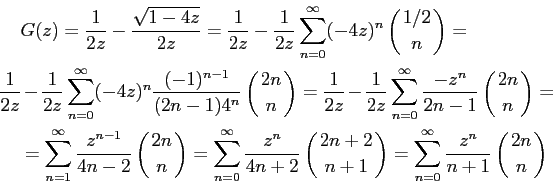
\includegraphics[width=\textwidth]{katalan}

Таким образом, коэффициент при $x^n$ в выражении $xf(x)$ равен $\frac{C^{n-1}_{2n-2}}{n};$. Это коэффициент для $T_{n-1}$. 

Следовательно, для $T_n$ получаем коэффициент $\frac{C^{n}_{2n}}{n+1}.$

\subsubsection{Задачи}
\textbf{Задача}. Докажите рекуррентное соотношение для чисел Каталана.

$\\$
Рассмотрим $2(n+1)$ скобок. Возьмем самую левую скобку и закрывающую ее правую. Пусть внутри них будет $k$ скобок. Тогда вне их будет $n-k$ скобок. Внутри них будет $T_k$ вариантов. Вне их будет $T_{n-k}$ вариантов. И так как $k \in [0, n]$, то, суммируя, получаем исходное соотношение (только нужно перестроить индексы для $T_n$, а не $T_{n+1}$).

$\\$
\textbf{Задача}. Найдите число $A_n$ количества триангуляций выпуклого $n$-угольника, то есть таких разбиений $n$-угольника на треугольники диагоналями, что диагонали пересекаются только в вершинах $n$-угольника.

$\\$
Зафикисируем одну сторону, которую назовем основанием. Другие две стороны треугольника для него --- это либо две диагонали, либо сторона + диагональ. Треугольник с основанием делит исходный многоугольник на два многоугольника поменьше, внутри которых могут быть свои разбиения.

Когда две другие стороны треугольника --- это сторона + диагональ, то отсекается многоугольник размера $n+1$, и таких случаев только два: для стороны слева и стороны справа.

Когда две другие стороны треугольника --- это две диагонали, то слева отсекается многоугольник размера $k$, а справа --- размера $n-2$.

Таким образом получаем рекуррентное соотношение:
$$A_n = A_0A_{n-1} + A_3A_{n-2} + A_4A_{n-3} + ... + A_4A_{n-3} + A_3A_{n-2} + A_0A_{n-1}$$
Если предположить, что $A_2 = 1$, то легким движением руки делаем замену $A_0$ на $A_2$:
$$A_n = A_2A_{n-1} + A_3A_{n-2} + A_4A_{n-3} + ... + A_4A_{n-3} + A_3A_{n-2} + A_2A_{n-1} = \sum\limits_{k=2}^{n-1} A_k \cdot A_{n-k+1}, n \geqslant 3.$$

Это очень похоже на рекуррентное соотношение для чисел Каталана, только со сдвигом: $A_2 = T_0, A_3 = T_1$.
$$A_3 = 1$$
$$A_4 = A_2A_3 + A_3A_2 = 2$$
$$A_5 = A_2A_4 + A_3A_3 + A_4A_2 = 5$$
$$A_6 = A_2A_5 + A_3A_4 + A_4A_3 + A_5A_2 = 14$$

Тогда как для чисел Каталана:
$$T_0 = T_1 = 1$$
$$T_2 = T_0T_1 + T_1T_0 = 2$$
$$T_3 = T_0T_2 + T_1T_1 + T_2T_0 = 5$$
$$T_4 = T_0T_3 + T_1T_2 + T_2T_1 + T_3T_0 = 14$$
Таким образом, из-за того, что $A_n$ позже "стартует", имеем сдвиг $A_n = T_{n-2}$ --- и не важно, что мы потеряли первые значения, а не последние: в итоге это оказывается равнозначным.

Но зависимость нужно доказать. Базу индукции мы доказали, нужно проверить переход. Докажем его для $k=n$ (предположив, что для $k-1$ у нас все правильно):
$$A_n = \sum\limits_{k=2}^{n-1} A_k \cdot A_{n-k+1} = \sum\limits_{k=2}^{n-1} T_{k-2} \cdot T_{n-k-1} = \sum\limits_{k=0}^{n-3} T_{k} \cdot T_{n-3-k} = T_{n-2}.$$
TODO: не очень понял про индукцию.

$\\$
\textbf{Задача}. Докажите тождество $4^n = \sum\limits_{i=0}^n C_{2i}^{i} \cdot C_{2(n-i)}^{n-i}$.

$\\$
Выпишем производящую функцию левой и правой частей равенства.

Ясно, что производящая функция $f(x)$ последовательности $a_n=4^n$ имеет вид $f(x) = 1+4x+4^2x^2+ \ldots = (1-4x)^{-1}$. 

Теперь рассмотрим производящую функцию $g(x)$ последовательности $g(x) =C_{2n}^n$. Нам необходимо доказать, что $f(x) = g^2(x)$. Значит, $g(x)$ должно быть равно $\frac{1}{(1 - 4x)^{\frac{1}{2}}}$. Если мы докажем, что коэффициенты ряда $\frac{1}{(1 - 4x)^{\frac{1}{2}}}$ равны $C_{2n}^n$, то все доказано. Имеем:
$$C_{-\frac{1}{2}}^n  = \frac{(-\frac{1}{2})(-\frac{3}{2})\ldots (-\frac{2n-1}{2})}{n!} = \frac{(-1)^n \cdot 1\cdot 3 \cdot \ldots \cdot (2n-1)}{2^n\cdot n!},$$
$$(-4)^n C_{-\frac{1}{2}}^n  = (-1)^n 4^n \frac{(-1)^n \cdot 1\cdot 3 \cdot \ldots \cdot (2n-1)}{2^n\cdot n!} = \frac{2^n \cdot 1\cdot 3 \cdot \ldots \cdot (2n-1) }{n!} =$$
$$\frac{2^n \cdot (2n)!}{n! \cdot 2 \cdot 4 \cdot \ldots \cdot 2n} = \frac{2n!}{n!n!} = C_{2n}^n$$

$\\$
\textbf{Задача}. Вычислите сумму $(C_n^0)^2-(C_n^1)^2+\ldots+(-1)^n(C_n^n)^2.$

$\\$
Перепишем выражение в виде $C_n^0 C_n^n -C_n^1 C_n^{n-1}+\ldots+(-1)^n C_n^n C_n^0.$

Рассмотрим производящую функцию $f(x)$ последовательности $a_k = C_n^0 C_n^k -C_n^1 C_n^{k-1}+\ldots+(-1)^k C_n^k C_n^0.$ Функция $f(x)$ является произведением функций $\sum_{k=0}^n C_n^k x^k = (1+x)^n$ и $\sum_{k=0}^n (-1)^k C_n^k x^k = (1-x)^{n}$.

Следовательно, $f(x) = (1+x)^n \cdot (1-x)^n = (1-x^2)^n$.

Следовательно, $a_n = \begin{cases} (-1)^kC_{2k}^k , \mbox{ если }  n=2k \\ 0, \mbox{ если }  n=2k+1 \end{cases}$.

\subsection{Задачи}
\textbf{Задача}. Найти сумму $\sum\limits_{n=0}^{\infty}\frac{F_n}{2^n},$ где $F_n$ --- числа Фибоначчи, $F_0 = F_1 = 1$.

$\\$
Так как $\frac{1}{2} < 0{,}612$, то число $\frac{1}{2}$ можно подставлять в ряд $\sum\limits_{n=0}^{\infty} F_n \cdot x^n = \frac{1}{1-x-x^2}$. Мы получаем, что $\sum\limits_{n=0}^{\infty}\frac{F_n}{2^n} = \frac{1}{1-\frac{1}{2}-\frac{1}{4}} = \frac{1}{\frac{1}{4}}=4.$.

$\\$
\textbf{Задача}. Найти значение $C_{-\frac{1}{3}}^5$.

$\\$
$$C_{-\frac{1}{3}}^5 = \frac{(-\frac{1}{3})(-\frac{4}{3})(-\frac{7}{3})(-\frac{10}{3})(-\frac{13}{3})}{5!} = - \frac{4\cdot 7\cdot 10 \cdot 13}{3^5\cdot 5!} = - \frac{ 7 \cdot 13}{3^5\cdot 3} = -\frac{91}{3^6} = -\frac{91}{729}.$$

$\\$
\textbf{Задача}. Вычислить сумму ряда $\sum\limits_{n=0}^{\infty}\frac{a_n}{2^n},$ где $a_0=7, a_1 = 12, a_n = a_{n-1}+a_{n-2}$.

$\\$
Рекуррентное соотношение для последовательности $a_n$ совпадает с рекуррентным соотношением для чисел Фибоначчи. 

Следовательно, $a_n = C_1 \left(\frac{1+\sqrt{5}}{2}\right)^n + C_2 \left( \frac{1-\sqrt{5}}{2} \right)^n$

Как и в случае чисел Фибоначчи, радиус сходимости степенного ряда приблизительно равен $0,612$, и поэтому для $\frac{1}{2}$ значение суммы имеет смысл.

Аналогично числам Фибоначчи, мы получаем соотношение:

$$x^2f(x) + xf(x) = f(x) +a_0x-a_0-a_1x$$
$$f(x) = \frac{a_0+(a_1-a_0)x}{1-x-x^2} = \frac{7+5x}{1-x-x^2}$$
$$f(\frac{1}{2}) = \frac{7+\frac{5}{2}}{1-\frac{1}{2}-\frac{1}{4}}=\frac{19}{2} : \frac{1}{4} = 38$$

$\\$
\textbf{Задача}. Сколько существует способов разместить числа $1,2,...,20$ в виде массива размера $2 \times 10$ так, чтобы и строки, и столбцы массива были упорядочены по возрастанию слева направо и сверху вниз? Пример такой таблицы:
$$\begin{pmatrix} 1& 2 &4& 5& 8 & 10 & 11 & 14 & 16& 18 \\ 3& 6& 7 & 9 & 12 & 13 & 15 & 17 & 19 & 20 \end{pmatrix}$$

$\\$
Построим биекцию между данной таблицей и сбалансированной последовательностей открывающих и закрывающих скобок. А именно, на каждое место, соответствующее числу в верхней строке поставим открывающую скобку, а на нижнее --- закрывающую. К примеру, данной таблице соответствует последовательность $(()(())()(())()()())$.

Следовательно, количество таких способов равно $T_{10} = \frac{20!}{10!\cdot 10! \cdot 11} = 16796$.

$\\$
\textbf{Задача}. Вычислите сумму $\sum_{s=0}^{100}(-1)^s C_{30+s}^sC_{100}^{100-s}.$

$\\$
Найдём производящую функцию $f(x)$ последовательности $a_n = \sum\limits_{s=0}^{n}(-1)^s C_{30+s}^sC_{n}^{n-s}$.

Ясно, что $f(x) = g(x)h(x)$:

$g(x)$ --- производящая функция для последовательности $b_n=(-1)^n C_{30+n}^n$.

$h(x)$ --- производящая функция для последовательности $c_n=C_{100}^n$, $0 \leq n \leq 100$.

В итоге имеем:

$$(-1)^n C_{30+n}^n  = (-1)^n\frac{(30+n)(30+n-1)\ldots (31)}{n!} = \frac{(-30-n)(-30-n+1)\ldots(-31)}{n!}  = C_{-31}^n$$

$$g(x) = \sum_{n=0}^{\infty} (-1)^n C_{30+n}^n x^n = \sum_{n=0}^{\infty} C_{-31}^{n} x^n = (1+x)^{-31}$$

$$h(x) = \sum_{n=0}^{100} C_{100}^n x^n = (1+x)^{100}$$

$$g(x)\cdot h(x) = (1+x)^{69}$$

Следовательно, коэффициент при степени $a^{100}$ равен $0$.

\end{document}